\documentclass[a4paper]{article}

\def\npart {II}
\def\nterm {Lent}
\def\nyear {2017}
\def\nlecturer {H. S. Reall}
\def\ncourse {Statistical Physics}
\def\nlectures {MWF.12}

% Imports
\ifx \nextra \undefined
  \usepackage[pdftex,
    hidelinks,
    pdfauthor={Dexter Chua},
    pdfsubject={Cambridge Maths Notes: Part \npart\ - \ncourse},
    pdftitle={Part \npart\ - \ncourse},
  pdfkeywords={Cambridge Mathematics Maths Math \npart\ \nterm\ \nyear\ \ncourse}]{hyperref}
  \title{Part \npart\ - \ncourse}
\else
  \usepackage[pdftex,
    hidelinks,
    pdfauthor={Dexter Chua},
    pdfsubject={Cambridge Maths Notes: Part \npart\ - \ncourse\ (\nextra)},
    pdftitle={Part \npart\ - \ncourse\ (\nextra)},
  pdfkeywords={Cambridge Mathematics Maths Math \npart\ \nterm\ \nyear\ \ncourse\ \nextra}]{hyperref}

  \title{Part \npart\ - \ncourse \\ {\Large \nextra}}
\fi

\author{Lectured by \nlecturer \\\small Notes taken by Dexter Chua}
\date{\nterm\ \nyear}

\usepackage{alltt}
\usepackage{amsfonts}
\usepackage{amsmath}
\usepackage{amssymb}
\usepackage{amsthm}
\usepackage{booktabs}
\usepackage{caption}
\usepackage{enumitem}
\usepackage{fancyhdr}
\usepackage{graphicx}
\usepackage{mathtools}
\usepackage{microtype}
\usepackage{multirow}
\usepackage{pdflscape}
\usepackage{pgfplots}
\usepackage{siunitx}
\usepackage{tabularx}
\usepackage{tikz}
\usepackage{tkz-euclide}
\usepackage[normalem]{ulem}
\usepackage[all]{xy}

\pgfplotsset{compat=1.12}

\pagestyle{fancyplain}
\lhead{\emph{\nouppercase{\leftmark}}}
\ifx \nextra \undefined
  \rhead{
    \ifnum\thepage=1
    \else
      \npart\ \ncourse
    \fi}
\else
  \rhead{
    \ifnum\thepage=1
    \else
      \npart\ \ncourse\ (\nextra)
    \fi}
\fi
\usetikzlibrary{arrows}
\usetikzlibrary{decorations.markings}
\usetikzlibrary{decorations.pathmorphing}
\usetikzlibrary{positioning}
\usetikzlibrary{fadings}
\usetikzlibrary{intersections}
\usetikzlibrary{cd}

\newcommand*{\Cdot}{\raisebox{-0.25ex}{\scalebox{1.5}{$\cdot$}}}
\newcommand {\pd}[2][ ]{
  \ifx #1 { }
    \frac{\partial}{\partial #2}
  \else
    \frac{\partial^{#1}}{\partial #2^{#1}}
  \fi
}

% Theorems
\theoremstyle{definition}
\newtheorem*{aim}{Aim}
\newtheorem*{axiom}{Axiom}
\newtheorem*{claim}{Claim}
\newtheorem*{cor}{Corollary}
\newtheorem*{defi}{Definition}
\newtheorem*{eg}{Example}
\newtheorem*{fact}{Fact}
\newtheorem*{law}{Law}
\newtheorem*{lemma}{Lemma}
\newtheorem*{notation}{Notation}
\newtheorem*{prop}{Proposition}
\newtheorem*{thm}{Theorem}

\renewcommand{\labelitemi}{--}
\renewcommand{\labelitemii}{$\circ$}
\renewcommand{\labelenumi}{(\roman{*})}

\let\stdsection\section
\renewcommand\section{\newpage\stdsection}

% Strike through
\def\st{\bgroup \ULdepth=-.55ex \ULset}

% Maths symbols
\newcommand{\bra}{\langle}
\newcommand{\ket}{\rangle}

\newcommand{\N}{\mathbb{N}}
\newcommand{\Z}{\mathbb{Z}}
\newcommand{\Q}{\mathbb{Q}}
\renewcommand{\H}{\mathbb{H}}
\newcommand{\R}{\mathbb{R}}
\newcommand{\C}{\mathbb{C}}
\newcommand{\Prob}{\mathbb{P}}
\renewcommand{\P}{\mathbb{P}}
\newcommand{\E}{\mathbb{E}}
\newcommand{\F}{\mathbb{F}}
\newcommand{\cU}{\mathcal{U}}
\newcommand{\RP}{\mathbb{RP}}
\newcommand{\CP}{\mathbb{CP}}

\newcommand{\ph}{\,\cdot\,}

\DeclareMathOperator{\sech}{sech}
\DeclareMathOperator{\cosech}{cosech}
\DeclareMathOperator{\cosec}{cosec}

\DeclareMathOperator{\covol}{covol}
\DeclareMathOperator{\vol}{vol}

\let\Im\relax
\let\Re\relax
\DeclareMathOperator{\Im}{Im}
\DeclareMathOperator{\Re}{Re}
\DeclareMathOperator{\im}{im}
\DeclareMathOperator{\image}{image}
\DeclareMathOperator{\Ann}{Ann}

\DeclareMathOperator*{\res}{res}
\DeclareMathOperator{\Res}{Res}
\DeclareMathOperator{\Ind}{Ind}

\DeclareMathOperator{\tr}{tr}
\DeclareMathOperator{\diag}{diag}
\DeclareMathOperator{\rank}{rank}
\DeclareMathOperator{\card}{card}
\DeclareMathOperator{\spn}{span}
\DeclareMathOperator{\adj}{adj}

\DeclareMathOperator{\erf}{erf}
\DeclareMathOperator{\erfc}{erfc}

\DeclareMathOperator{\ord}{ord}
\DeclareMathOperator{\Sym}{Sym}

\DeclareMathOperator{\sgn}{sgn}
\DeclareMathOperator{\orb}{orb}
\DeclareMathOperator{\stab}{stab}
\DeclareMathOperator{\ccl}{ccl}

\DeclareMathOperator{\lcm}{lcm}
\DeclareMathOperator{\hcf}{hcf}

\DeclareMathOperator{\Int}{Int}
\DeclareMathOperator{\id}{id}

\DeclareMathOperator{\betaD}{beta}
\DeclareMathOperator{\gammaD}{gamma}
\DeclareMathOperator{\Poisson}{Poisson}
\DeclareMathOperator{\binomial}{binomial}
\DeclareMathOperator{\multinomial}{multinomial}
\DeclareMathOperator{\Bernoulli}{Bernoulli}
\DeclareMathOperator{\like}{like}

\DeclareMathOperator{\var}{var}
\DeclareMathOperator{\cov}{cov}
\DeclareMathOperator{\bias}{bias}
\DeclareMathOperator{\mse}{mse}
\DeclareMathOperator{\corr}{corr}

\DeclareMathOperator{\otp}{otp}
\DeclareMathOperator{\dom}{dom}

\DeclareMathOperator{\Root}{Root}
\DeclareMathOperator{\supp}{supp}
\DeclareMathOperator{\rel}{rel}
\DeclareMathOperator{\Hom}{Hom}
\DeclareMathOperator{\Aut}{Aut}
\DeclareMathOperator{\Gal}{Gal}
\DeclareMathOperator{\Mat}{Mat}
\DeclareMathOperator{\End}{End}
\DeclareMathOperator{\Char}{char}
\DeclareMathOperator{\ev}{ev}
\DeclareMathOperator{\St}{St}
\DeclareMathOperator{\Lk}{Lk}
\DeclareMathOperator{\disc}{disc}
\DeclareMathOperator{\Isom}{Isom}
\DeclareMathOperator{\length}{length}
\DeclareMathOperator{\energy}{energy}
\DeclareMathOperator{\area}{area}
\DeclareMathOperator{\Syl}{Syl}
\DeclareMathOperator{\cl}{cl}
\DeclareMathOperator{\fix}{fix}

\newcommand{\GL}{\mathrm{GL}}
\newcommand{\SL}{\mathrm{SL}}
\newcommand{\PGL}{\mathrm{PGL}}
\newcommand{\PSL}{\mathrm{PSL}}
\newcommand{\PSU}{\mathrm{PSU}}
\newcommand{\Or}{\mathrm{O}}
\newcommand{\SO}{\mathrm{SO}}
\newcommand{\U}{\mathrm{U}}
\newcommand{\SU}{\mathrm{SU}}

\renewcommand{\d}{\mathrm{d}}
\newcommand{\D}{\mathrm{D}}

\tikzset{->/.style = {decoration={markings,
                                  mark=at position 1 with {\arrow[scale=2]{latex'}}},
                      postaction={decorate}}}
\tikzset{<-/.style = {decoration={markings,
                                  mark=at position 0 with {\arrowreversed[scale=2]{latex'}}},
                      postaction={decorate}}}
\tikzset{<->/.style = {decoration={markings,
                                   mark=at position 0 with {\arrowreversed[scale=2]{latex'}},
                                   mark=at position 1 with {\arrow[scale=2]{latex'}}},
                       postaction={decorate}}}
\tikzset{->-/.style = {decoration={markings,
                                   mark=at position #1 with {\arrow[scale=2]{latex'}}},
                       postaction={decorate}}}
\tikzset{-<-/.style = {decoration={markings,
                                   mark=at position #1 with {\arrowreversed[scale=2]{latex'}}},
                       postaction={decorate}}}

\tikzset{circ/.style = {fill, circle, inner sep = 0, minimum size = 3}}
\tikzset{mstate/.style={circle, draw, blue, text=black, minimum width=0.7cm}}

\definecolor{mblue}{rgb}{0.2, 0.3, 0.8}
\definecolor{morange}{rgb}{1, 0.5, 0}
\definecolor{mgreen}{rgb}{0.1, 0.4, 0.2}
\definecolor{mred}{rgb}{0.5, 0, 0}

\def\drawcirculararc(#1,#2)(#3,#4)(#5,#6){%
    \pgfmathsetmacro\cA{(#1*#1+#2*#2-#3*#3-#4*#4)/2}%
    \pgfmathsetmacro\cB{(#1*#1+#2*#2-#5*#5-#6*#6)/2}%
    \pgfmathsetmacro\cy{(\cB*(#1-#3)-\cA*(#1-#5))/%
                        ((#2-#6)*(#1-#3)-(#2-#4)*(#1-#5))}%
    \pgfmathsetmacro\cx{(\cA-\cy*(#2-#4))/(#1-#3)}%
    \pgfmathsetmacro\cr{sqrt((#1-\cx)*(#1-\cx)+(#2-\cy)*(#2-\cy))}%
    \pgfmathsetmacro\cA{atan2(#2-\cy,#1-\cx)}%
    \pgfmathsetmacro\cB{atan2(#6-\cy,#5-\cx)}%
    \pgfmathparse{\cB<\cA}%
    \ifnum\pgfmathresult=1
        \pgfmathsetmacro\cB{\cB+360}%
    \fi
    \draw (#1,#2) arc (\cA:\cB:\cr);%
}
\newcommand\getCoord[3]{\newdimen{#1}\newdimen{#2}\pgfextractx{#1}{\pgfpointanchor{#3}{center}}\pgfextracty{#2}{\pgfpointanchor{#3}{center}}}

\def\Xint#1{\mathchoice
   {\XXint\displaystyle\textstyle{#1}}%
   {\XXint\textstyle\scriptstyle{#1}}%
   {\XXint\scriptstyle\scriptscriptstyle{#1}}%
   {\XXint\scriptscriptstyle\scriptscriptstyle{#1}}%
   \!\int}
\def\XXint#1#2#3{{\setbox0=\hbox{$#1{#2#3}{\int}$}
     \vcenter{\hbox{$#2#3$}}\kern-.5\wd0}}
\def\ddashint{\Xint=}
\def\dashint{\Xint-}


\begin{document}
\maketitle
{\small
  \noindent\emph{Part IB Quantum Mechanics and ``Multiparticle Systems'' from Part II Principles of Quantum Mechanics are essential}

  \vspace{10pt}
  \noindent\textbf{Fundamentals of statistical mechanics}\\
  Microcanonical ensemble. Entropy, temperature and pressure. Laws of thermodynamics. Example of paramagnetism. Boltzmann distribution and canonical ensemble. Partition function. Free energy. Specific heats. Chemical Potential. Grand Canonical Ensemble.\hspace*{\fill} [5]

  \vspace{10pt}
  \noindent\textbf{Classical gases}\\
  Density of states and the classical limit. Ideal gas. Maxwell distribution. Equipartition of energy. Diatomic gas. Interacting gases. Virial expansion. Van der Waal's equation of state. Basic kinetic theory.\hspace*{\fill} [3]

  \vspace{10pt}
  \noindent\textbf{Quantum gases}\\
  Density of states. Planck distribution and black body radiation. Debye model of phonons in solids. Bose-Einstein distribution. Ideal Bose gas and Bose-Einstein condensation. Fermi-Dirac distribution. Ideal Fermi gas. Pauli paramagnetism.\hspace*{\fill}[8]

  \vspace{10pt}
  \noindent\textbf{Thermodynamics}\\
  Thermodynamic temperature scale. Heat and work. Carnot cycle. Applications of laws of thermodynamics. Thermodynamic potentials. Maxwell relations.\hspace*{\fill} [4]

  \vspace{10pt}
  \noindent\textbf{Phase transitions}\\
  Liquid-gas transitions. Critical point and critical exponents. Ising model. Mean field theory. First and second order phase transitions. Symmetries and order parameters.\hspace*{\fill} [4]%
}

\tableofcontents
\setcounter{section}{-1}
\section{Introduction}
In previous physics courses, we mostly focused on ``microscopic'' physics. We looked at the interaction of atoms, electrons etc. We now want to look at more macroscopic things, when we have lots of atoms, and lots of molecules. The aim of the course is translate microscopic laws of physics into macroscopic laws of physics.

By ``macroscopic'', we mean a system that is made of many particles. For example, $\SI{12}{\gram}$ of Carbon-12 contains $6 \times 10^{23}$ atoms, known as a mole. This number is very big. This is the key ingredient we are going to talk about in this course. How do we go about doing that? We might want to write down the Schr\"odinger equation for all water particles in a bottle, and then see how it evolves in time, and then predict how water evolves. But this is, obviously, hopeless. Even if we have two atoms, it is very hard to solve the Schr\"odinger equation, let alone $10^{23}$. But we don't have to. We don't have to have a complete description of the molecules if we want to know how the water behaves. It doesn't matter if we swap around two water molecules. We just want to know about macroscopic properties of the substance.

For example, temperature is something we can ask about a system, and this is a property of a system. It doesn't make sense to ask the temperature of a particle.

Historically, one reason to study statistical physics is that we can use it to test our microscopic laws of matter. For example, this is how quantum mechanics was discovered. Nowadays, techniques in statistical physics have many applications. In addition to studying, say, condensed matter physics, they can be used to do many other things like studying black holes, or biology!

\section{Fundamentals of statistical mechanics}
\subsection{Microcanonical ensemble}
The general setting in this section is that we have an isolated system containing $N$ particles, where $N$ is a Large Number\textsuperscript{TM}.

\begin{eg}
  A gas in a box can be considered to be an isolated system with many particles.
\end{eg}

\begin{defi}[Microstate]\index{microstate}
  The \emph{microstate} of a system is the actual (quantum) state of the system. This gives a complete description of the system.
\end{defi}

As one would expect, the microstate is very complicated and infeasible to describe, especially when we have \emph{many} particles. In statistical physics, we observe that many microstates are indistinguishable macroscopically. Thus, we only take note of some macroscopically interesting quantities, and use these macroscopic quantities to put a probability distribution on the microstates.

More precisely, we let $\{\bket{n}\}$ be a basis of normalized eigenstates, say
\[
  \hat{H}\bket{n} = E_n \bket{n}.
\]
We let $p(n)$ be the probability that the microstate is $\bket{n}$. Note that this probability is not the quantum probability we usually meet, but just something reflecting our ignorance.

Given such probabilities, we can define the expectation of an operator in the least imaginative way:
\begin{defi}[Expectation value]\index{expectation value}
  Given a probability distribution $p(n)$ on the states, the expectation value of an operator $\mathcal{O}$ is
  \[
    \bra \mathcal{O}\ket = \sum_n p(n) \brak{n}\mathcal{O}\bket{n}.
  \]
\end{defi}
If one knows about density operators, we can describe the system as a mixed state with density operator
\[
  \rho = \sum_n p(n) \bket{n}\brak{n}.
\]
There is an equivalent way of looking at this. We can consider an \term{ensemble} consisting of $W \gg 1$ independent copies of our system such that $Wp(m)$ many copies are in the microstate $\bket{n}$. Then the expectation is just the average over the ensemble.

We will further assume our system is in \term{equilibrium}, ie. the probability distribution $p(n)$ does not change in time. So in particular $\bra O\ket$ is independent of time. Of course, this does not mean the particles stop moving. The particles are still whizzing around. It's just that the statistical distribution does not change. In this course, we will mostly be talking about equilibrium systems. When we get out of equilibrium, things become very complicated.

The idea of statistical physics is that we have some partial knowledge about the system. For example, we might know its total energy. The microstates that are compatible with this partial knowledge are called \emph{accessible}\index{accessible state}. The \term{fundamental assumption of statistical mechanics} is then
\begin{significant}
  An isolated system in equilibrium is equally likely to be in any of the accessible microstates.
\end{significant}
This is an assumption we make, and we will see that it works very well.

Thus, different probability distributions, or different ensembles, are distinguished by the partial knowledge we know.
\begin{defi}[Microcanonical ensemble]\index{microcanonical ensemble}
  In a \emph{microcanonical ensemble}, we know the energy is between $E$ and $E + \delta E$, where $\delta E$ Is the accuracy of our measuring device. The accessible microstates are those with energy $E \leq E_n \leq E + \delta E$. We let $\Omega(E)$ be the number of such states.
\end{defi}
In practice, $\delta E$ is much much larger than the spacing of energy levels, and so $\Omega(E) \gg 1$.

Note that we are working with a quantum system here, so the possible systems is discrete, and so it makes sense to count the number of systems. We need to do more work if we want to do this classically.

\begin{eg}
  Suppose we have $N = 10^{23}$ particles, and each particle can occupy two states $\bket{\uparrow}$ and $\bket{\downarrow}$, which have the same energy $\varepsilon$. Then we always have $N\varepsilon$ total energy, and we have
  \[
    \Omega(N\varepsilon) = 2^{10^{23}}.
  \]
  This is a fantastically huge, mind-boggling number. This is the kind of number we are talking about.
\end{eg}

By the fundamental assumption, we have
\[
  p(n) =
  \begin{cases}
    \frac{1}{\Omega(E)} & \text{if } E \leq E_n \leq E + \delta E\\
    0 & \text{otherwise}
  \end{cases}
\]
This probability distribution defines what is known as as the microcanonical ensemble.

Since this $\Omega(E)$ is huge, we want something smaller, one that is linear in $N$. So we take the log

\begin{defi}[Boltzmann entropy]\index{Boltzmann entropy}\index{entropy}
  The \emph{(Boltzmann) entropy} is defined as
  \[
    S(E) = k \log \Omega(E),
  \]
  where $k = \SI{1.381e-23}{\joule\per\kelvin}$ is \term{Boltzmann's constant}\index{$k$}.
\end{defi}
This annoying constant $k$ is necessary because when people started doing thermodynamics, they didn't know about statistical physics, and picked weird conventions.

As we have seen previously, we expect $\Omega(E) \sim e^N$. So we would expect $S(E) \sim kN$, and this is why the entropy is more convenient.

Notice that we wrote our expressions as $S(E)$, instead of $S(E, \delta E)$. It turns out the value of $\delta E$ doesn't really matter. We know that $\Omega(E)$ will scale approximately linearly with $\delta E$. So if we, say, double $\delta E$, then $S(E)$ will increase by $k \log 2$, which is incredibly tiny compared to $S(E) = k \log \Omega(E)$. So it doesn't matter which value of $\delta E$ we pick.

Even if you are not so convinced that multiplying $10^{10^{23}}$ by a factor of $2$ or adding $\log 2$ to $10^{23}$ do not really matter, you should be reassured that at the end, we will rarely talk about $\Omega(E)$ or $S(E)$ itself. Instead, we will often divide two different $\Omega$'s to get probabilities, or differentiate $S$ to get other interesting quantities, and in these cases, those factors do not matter.


The second nice property of the entropy is that it is additive --- if we have two \emph{non-interacting} systems with energies $E_{(1)}, E_{(2)}$. Then the total number of states of the combined system is
\[
  \Omega(E_{(1)}, E_{(2)}) = \Omega_{1}(E_{(1)})\Omega_{2} (E_{(2)}).
\]
So when we take the logarithm, we find
\[
  S(E_{(1)}, E_{(2)}) = S(E_{(1)}) + S(E_{(2)}).
\]
This is for systems that do not interact with each other.

\subsubsection*{Interacting systems}
Suppose we bring the two systems together, and let them exchange energy. Then the energy of the individual systems is no longer fixed, and only the total energy
\[
  E_{\mathrm{total}} = E_{(1)} + E_{(2)}
\]
is fixed. Then we find that
\[
  \Omega(E_{\mathrm{total}}) = \sum_{E_i} \Omega_1(E_i) \Omega_2(E_{\mathrm{total}} - E_i),
\]
where we sum over all possible energy levels of the first system. In terms of the entropy of the system, we have
\[
  \Omega(E_{\mathrm{total}}) = \sum_{E_i} \exp\left(\frac{S_1(E_i)}{k} + \frac{S_2(E_{\mathrm{total}} - E_i)}{k}\right)
\]
We can be a bit more precise with what the sum means. We are not summing over all eigenstates. Recall that we have previously fixed an accuracy $\delta E$. So we can imagine dividing the whole energy spectrum into chunks of size $\delta E$, and here we are summing over the chunks.

We know that $S_{1, 2}/k \sim N_{1, 2} \sim 10^{23}$, which is a ridiculously large number. So the sum is overwhelmingly dominated by the term with the largest exponent. Suppose this is maximized when $E_i = E_*$. Then we have
\[
  S(E_{\mathrm{total}}) = k \log \Omega(E_{\mathrm{total}}) \approx S_1(E_*) + S_2(E_{\mathrm{total}} - E_*).
\]
Again, we are not claiming that only the factor coming from $E_*$ has significant contribution. Maybe one or two energy levels next to $E_*$ are also very significant, but taking these into account will only multiply $\Omega(E_{\mathrm{total}})$ by a (relatively) small constant, hence contributes a small additive factor to $S(E_{\mathrm{total}})$, which can be neglected.

Now given any $E_{(1)}$, what is the probability that the actual energy of the first system is $E_{(1)}$? For convenience, we write $E_{(2)} = E_{\mathrm{total}} = E_{(1)}$, the energy of the second system. Then the probability desired is
\[
  \frac{\Omega_1(E_{(1)})\Omega_2(E_{(2)})}{\Omega(E_{\mathrm{total}})} = \exp\left(\frac{1}{k}\left(S_1(E_{(1)}) + S_2(E_{(2)}) - S(E_{\mathrm{total}})\right)\right).
\]
Again recall that the numbers at stake are unimaginably huge. So if $S_1(E_{(1)}) + S_2(E_{(2)})$ is even slightly different from $S(E_{\mathrm{total}})$, then the probability is effectively zero. And by above, for the two quantities to be close, we need $E_{(1)} = E_*$. So for all practical purposes, the value of $E_{(1)}$ is fixed into $E_*$.

Now imagine we prepare two systems separately with energies $E_{(1)}$ and $E_{(2)}$ such that $E_{(1)} \not= E_*$, and then bring the system together, then we are no longer in equilibrium. $E_{(1)}$ will change until it takes value $E_*$, and then entropy of the system will increase from $S_1(E_{(1)}) + S_2(E_{(2)})$ to $S_1(E_*) + S_2(E_{\mathrm{total}} - E_*)$. In particular, the entropy increases.
\begin{law}[Second law of thermodynamics]\index{second law of thermodynamics}
  The entropy of an isolated system increases (or remains the same) in any physical process. In equilibrium, the entropy attains its maximum value.
\end{law}
This prediction is verified by virtually all observations of physics.

While our derivation did not show it is \emph{impossible} to violate the second law of thermodynamics, it is very very very very very very very very unlikely to be violated.

\subsubsection*{Temperature}
Having defined entropy, the next interesting thing we can define is the \emph{temperature}. We assume that $S$ is a smooth function in $E$. Then we can define the temperature as follows:
\begin{defi}[Temperature]\index{temperature}
  The \emph{temperature} is defined to be
  \[
    \frac{1}{T} = \frac{\d S}{\d E}.
  \]
\end{defi}
Why do we call this the temperature? Over the course, we will see that this quantity we decide to call ``temperature'' does behave as we would expect temperature to behave. Since there is no other ``standard'' definition of temperature we can compare this to, it would be difficult to give more direct justifications of this definition.

\begin{prop}
  Two interacting systems in equilibrium have the same temperature.
\end{prop}

\begin{proof}
  Recall that the equilibrium energy $E_*$ is found by maximizing
  \[
    S_1(E_i) + S_2(E_{\mathrm{total}} - E_i)
  \]
  over all possible $E_i$. Thus, at an equilibrium, the derivative of this expression has to vanish, and the derivative is exactly
  \[
    \left.\frac{\d S_1}{\d E}\right|_{E_{(1)} = E_*} - \left.\frac{\d S_i}{\d E} \right|_{E_{(2)} = E_{\mathrm{total}} - E_*} = 0
  \]
  So we need
  \[
    \frac{1}{T_1} = \frac{1}{T_2}.
  \]
  In other words, we need
  \[
    T_1 = T_2.
  \]
\end{proof}

Now suppose initially, our systems have different temperature. We would expect energy to flow from the hotter system to the cooler system. This is indeed the case.

\begin{prop}
  Suppose two systems with initial energies $E_{(1)}, E_{(2)}$ and temperatures $T_1, T_2$ are put into contact. If $T_1 > T_2$, then energy will flow form the first system to the second.
\end{prop}

\begin{proof}
  Since we are not in equilibrium, there must be some energy transfer from one system to the other. Suppose after time $\delta t$, the energy changes by
  \begin{align*}
    E_{(1)} & \mapsto E_{(1)} + \delta E\\
    E_{(2)} & \mapsto E_{(2)} - \delta E,
  \end{align*}
  keeping the total energy constant. Then the change in entropy is given by
  \[
    \delta S = \frac{\d S_1}{\d E} \delta E_{(1)} + \frac{\d S_2}{\d E} \delta E_{(2)} = \left(\frac{1}{T_1} - \frac{1}{T_2}\right) \delta E.
  \]
  By assumption, we know
  \[
    \frac{1}{T_1} - \frac{1}{T_2} < 0,
  \]
  but by the second law of thermodynamics, we know $\delta S$ must increase. So we must have $\delta E < 0$, ie. energy flows from the first system to the second.
\end{proof}
So this notion of temperature agrees with the basic properties of temperature we expect.

Note that, these properties we've derived only depends on the fact that $\frac{1}{T}$ is a monotonically decreasing function of $T$. In principle, we could have picked \emph{any} monotonically decreasing function of $T$, and set it to $\frac{\d S}{\d E}$. We will later see that this definition will agree with the other definitions of temperature we have previously seen, eg. via the ideal gas law, and so this is indeed the ``right'' one.

\subsubsection*{Heat capacity}
As we will keep on doing later, we can take different derivatives to get different interesting quantities. This time, we are going to get heat capacity. Recall that $T$ was a function of energy, $T = T(E)$. We will assume that we can invert this function, at least locally, to get $E$ as a function of $T$.
\begin{defi}[Heat capacity]\index{heat capacity}
  The \emph{heat capacity} of a system is
  \[
    C = \frac{\d E}{\d T}.
  \]
  The \term{specific heat capacity} is
  \[
    \frac{C}{\text{mass of system}}.
  \]
\end{defi}
The specific heat capacity is a property of the substance that makes up the system, and not how much stuff there is, as both $C$ and the mass scale linearly with the size of the system.

This is some quantity we can actually physically measure. We can measure the temperature with a thermometer, and it is usually not too difficult to see how much energy we pump into a system. Then by measuring the temperature change, we can figure out the heat capacity.

In doing so, we can indirectly measure the entropy, or at least the changes in entropy. Note that we have
\[
  \frac{\d S}{\d T} = \frac{\d S}{\d E} \frac{\d E}{\d T} = \frac{C}{T}.
\]
Integrating up, if the temperature changes from $T_1$ to $T_2$, we know
\[
  \Delta S = \int_{T_1}^{T_2} \frac{C(T)}{T}\;\d T.
\]
As promised, by measuring heat capacity experimentally, we can measure the change in entropy.

The heat capacity is useful in other ways. Recall that to find the equilibrium energy $E_*$, a necessary condition was that it satisfies
\[
  \frac{\d S_1}{\d E} - \frac{\d S_2}{\d E} = 0.
\]
However, we only know that the solution is an extrema, and not necessarily maximum. To figure out if it is the maximum, we take the second derivative. Note that for a single system, we have
\[
  \frac{\d^2 S}{\d E^2} = \frac{\d}{\d E} \left(\frac{1}{T}\right) = -\frac{1}{T^2 C}.
\]
Applying this to two systems, one can check that entropy is maximized at $E_{(1)} = E_*$ if $C_1, C_2 > 0$. The actual computations is left as an exercise on the first example sheet.

Let's look at some actual systems and try to calculate these quantities.
\begin{eg}
  Consider a $2$-state system, where we have $N$ non-interacting particles with fixed positions. Each particle is either in $\bket{\uparrow}$ or $\bket{\downarrow}$. We can think of these as spins, for example. These two states have different energies
  \[
    E_{\uparrow} = \varepsilon,\quad E_{\downarrow} = 0.
  \]
  We let $N_{\uparrow}$ and $N_{\downarrow}$ be the number of particles in $\bket{\uparrow}$ and $\bket{\downarrow}$ respectively. Then the total energy of the system is
  \[
    E = \varepsilon N_{\uparrow}.
  \]
  We want to calculate this quantity $\Omega(E)$. Here in this very contrived example, it is convenient to pick $\delta E < \varepsilon$, so that $\Omega(E)$ is just the number of ways of choosing $N_{\uparrow}$ particles from $N$. By basic combinatorics, we have
  \[
    \Omega(E) = \frac{N!}{N_{\uparrow}! (N - N_\uparrow)!},
  \]
  and
  \[
    S(E) = k \log \left(\frac{N!}{N_{\uparrow}! (N - N_\uparrow)!}\right).
  \]
  This is not an incredibly useful formula. Since we assumed that $N$ and $N_\uparrow$ are huge, we can use \term{Stirling's approximation}
  \[
    N! = \sqrt{2\pi N} N^N e^{-N} \left(1 + O\left(\frac{1}{N}\right)\right).
  \]
  Then we have
  \[
    \log N! = N \log N - N + \frac{1}{2}\log (2\pi N) + O\left(\frac{1}{N}\right).
  \]
  We just use the approximation three times to get
  \begin{align*}
    S(E) &= k\left(N \log N - N - N_\uparrow \log N_\uparrow + N_\uparrow - (N - N_\uparrow) \log(N - N_\uparrow) + N - N_\uparrow\right)\\
    &= -k \left((N - N_\uparrow) \log \left(\frac{N - N_\uparrow}{N}\right) + N_\uparrow \log\left(\frac{N_{\uparrow}}{N}\right)\right)\\
    &= -kN\left(\left(1 - \frac{E}{N\varepsilon}\right) \log\left(1 - \frac{E}{N\varepsilon}\right) + \frac{E}{N\varepsilon} \log\left(\frac{E}{N\varepsilon}\right)\right).
  \end{align*}
  This is better, but we can get much more out of it if we plot it:
  \begin{center}
    \begin{tikzpicture}
      \draw [->] (0, 0) -- (6, 0) node [right] {$E$};
      \draw [->] (0, 0) -- (0, 4) node [above] {$S(E)$};

      \draw [mblue, thick, domain=0.001:4.999] plot [smooth] (\x, {(-4.5) * ((1 - \x/5) * ln (1 - \x/5) + (\x / 5) * ln (\x / 5))});

      \node [left] at (0, 0) {$0$};
      \node [below] at (5, 0) {$N\varepsilon$};
      \node [below] at (2.5, 0) {$N\varepsilon/2$};
      \draw [dashed] (2.5, 0) -- (2.5, 3);

      \draw [dashed] (2.5, 3.119) -- (0, 3.119) node [left] {$Nk \log 2$};
    \end{tikzpicture}
  \end{center}
  The temperature is
  \[
    \frac{1}{T} = \frac{\d S}{\d T} = \frac{k}{\varepsilon} \log \left(\frac{N \varepsilon}{E} - 1\right),
  \]
  and we can invert to get
  \[
    \frac{N_{\uparrow}}{N} = \frac{E}{N\varepsilon} = \frac{1}{e^{\varepsilon /kT} + 1}.
  \]
  Suppose we get to control the temperature of the system, eg. if we put it with a heat reservoir. What happens as we vary our temperature?
  \begin{itemize}
    \item As $T \to 0$, we have $N_\uparrow \to 0$. So the states all try to go to the ground state.
    \item As $T \to \infty$, we find $N_\uparrow/N \to \frac{1}{2}$, and $E \to N\varepsilon/2$.
  \end{itemize}
  The second result is a bit weird. As $T \to \infty$, we might expect all things to go the maximum energy level, and not just half of them. What is happening?

  We can plot another graph, for $\frac{1}{T}$ vs $E$. The graph looks like
  \begin{center}
    \begin{tikzpicture}
      \draw [->] (0, 0) -- (6, 0) node [right] {$E$};
      \draw [->] (0, -2.5) -- (0, 2.5) node [above] {$\frac{1}{T}$};

      \draw [mblue, thick, domain=0.1:4.9] plot [smooth] (\x, {(-0.6) * (ln (\x) - ln (5 - \x))});

      \node [left] at (0, 0) {$0$};
      \node [below] at (5, 0) {$N\varepsilon$};
      \node [below] at (2.5, 0) {$N\varepsilon/2$};

    \end{tikzpicture}
  \end{center}
  We see that having energy $> N\varepsilon/2$ corresponds to negative temperature, and to go from positive temperature to negative temperature, we need to pass through infinite temperature. So in some sense, negative temperature is ``hotter'' than infinite temperature.

  What is going on? For negative $T$, we know $\Omega(E)$ is a decreasing function of energy. This is a very unusual situation. What we have in this system is that these particles are fixed, and have no kinetic energy. If we do have kinetic energy, then kinetic energy can be arbitrarily large. So there is no upper bound on $E$, and $\Omega(E)$ is usually an increasing function of $E$.

  Negative $T$ has indeed been observed experimentally. This requires setups where the kinetic energy is not so important in the range of energies we are talking about. One particular scenario where this is observed is in nuclear spins of crystals in magnetic fields. If we have a magnetic field, then naturally, most of the spins will align with the field. We now suddenly flip the field, and then most of the spins are anti-aligned, and this can give us a negative temperature state.

  Now we can't measure negative temperature by sticking a thermometer into the material and getting a negative answer. Something that \emph{can} be interestingly measured is the heat capacity
  \[
    C = \frac{\d E}{\d T} = \frac{N\varepsilon^2}{ kT^2 } \frac{e^{\varepsilon/kT}}{(e^{\varepsilon/kT} + 1)^2}.
  \]
  This again exhibits some peculiar properties. We begin by looking at a plot:
  \begin{center}
    \begin{tikzpicture}
      \draw [->] (0, 0) -- (6, 0) node [right] {$T$};
      \draw [->] (0, 0) -- (0, 4) node [above] {$C$};

      \draw [mblue, thick ] plot coordinates {(0.01,0.00000) (0.04,0.00000) (0.07,0.00102) (0.10,0.03632) (0.13,0.21581) (0.16,0.60094) (0.19,1.13589) (0.22,1.71794) (0.25,2.26083) (0.28,2.71418) (0.31,3.05901) (0.34,3.29686) (0.37,3.44009) (0.40,3.50519) (0.43,3.50895) (0.46,3.46653) (0.49,3.39067) (0.52,3.29165) (0.55,3.17751) (0.58,3.05435) (0.61,2.92675) (0.64,2.79804) (0.67,2.67060) (0.70,2.54609) (0.73,2.42564) (0.76,2.30996) (0.79,2.19945) (0.82,2.09433) (0.85,1.99462) (0.88,1.90026) (0.91,1.81111) (0.94,1.72699) (0.97,1.64766) (1.00,1.57290) (1.03,1.50244) (1.06,1.43606) (1.09,1.37350) (1.12,1.31453) (1.15,1.25893) (1.18,1.20647) (1.21,1.15697) (1.24,1.11022) (1.27,1.06605) (1.30,1.02429) (1.33,0.98478) (1.36,0.94739) (1.39,0.91196) (1.42,0.87839) (1.45,0.84654) (1.48,0.81631) (1.51,0.78760) (1.54,0.76031) (1.57,0.73436) (1.60,0.70966) (1.63,0.68614) (1.66,0.66373) (1.69,0.64237) (1.72,0.62198) (1.75,0.60252) (1.78,0.58393) (1.81,0.56617) (1.84,0.54918) (1.87,0.53292) (1.90,0.51735) (1.93,0.50244) (1.96,0.48815) (1.99,0.47445) (2.02,0.46130) (2.05,0.44868) (2.08,0.43656) (2.11,0.42492) (2.14,0.41372) (2.17,0.40295) (2.20,0.39259) (2.23,0.38262) (2.26,0.37302) (2.29,0.36376) (2.32,0.35484) (2.35,0.34624) (2.38,0.33795) (2.41,0.32994) (2.44,0.32221) (2.47,0.31475) (2.50,0.30753) (2.53,0.30056) (2.56,0.29382) (2.59,0.28731) (2.62,0.28100) (2.65,0.27490) (2.68,0.26899) (2.71,0.26326) (2.74,0.25772) (2.77,0.25235) (2.80,0.24714) (2.83,0.24209) (2.86,0.23719) (2.89,0.23243) (2.92,0.22782) (2.95,0.22334) (2.98,0.21899) (3.01,0.21477) (3.04,0.21066) (3.07,0.20667) (3.10,0.20280) (3.13,0.19902) (3.16,0.19536) (3.19,0.19179) (3.22,0.18832) (3.25,0.18494) (3.28,0.18165) (3.31,0.17844) (3.34,0.17532) (3.37,0.17228) (3.40,0.16932) (3.43,0.16644) (3.46,0.16362) (3.49,0.16088) (3.52,0.15820) (3.55,0.15559) (3.58,0.15305) (3.61,0.15056) (3.64,0.14814) (3.67,0.14577) (3.70,0.14346) (3.73,0.14120) (3.76,0.13899) (3.79,0.13684) (3.82,0.13474) (3.85,0.13268) (3.88,0.13067) (3.91,0.12870) (3.94,0.12678) (3.97,0.12490) (4.00,0.12307) (4.03,0.12127) (4.06,0.11951) (4.09,0.11779) (4.12,0.11611) (4.15,0.11446) (4.18,0.11284) (4.21,0.11126) (4.24,0.10972) (4.27,0.10820) (4.30,0.10672) (4.33,0.10526) (4.36,0.10384) (4.39,0.10244) (4.42,0.10107) (4.45,0.09973) (4.48,0.09842) (4.51,0.09713) (4.54,0.09587) (4.57,0.09463) (4.60,0.09341) (4.63,0.09222) (4.66,0.09105) (4.69,0.08990) (4.72,0.08877) (4.75,0.08767) (4.78,0.08658) (4.81,0.08552) (4.84,0.08447) (4.87,0.08345) (4.90,0.08244) (4.93,0.08145) (4.96,0.08047) (4.99,0.07952)};
      % map (\x -> (showFFloat (Just 2) x "", showFFloat (Just 5) (8 / (x*x) * exp (1/x) / (exp(1/x) + 1)^2) "")) [0.01,0.04..5]
      \node [left] at (0, 0) {$0$};

      \draw [dashed] (0.43, 0) node [below] {$T \sim \varepsilon/k$} -- (0.43, 3.50895);

    \end{tikzpicture}
  \end{center}
  Now the maximum $T$ is related to the microscopic $\varepsilon$. So we can use the macroscopic observation of $C$ to deduce something about the microscopic $\varepsilon$.

  Note that $C$ is proportional to $N$. As $T \to 0$, we have
  \[
    C \propto T^{-2} e^{-\varepsilon/kT},
  \]
  and this is a function that decreases very rapidly as $T \to 0$, and in fact this is one of the favorite examples in Analysis where all derivatives of the function at $0$ vanish. We will later see that this is due to the energy gap between the ground state and the first excited state.

  More interestingly, we see that the heat capacity vanishes at high temperature, but this is due to the peculiar property of the system at high temperature. In a general system, we expect the heat capacity to increase with temperature.

  How much of this is actually physical? The answer is ``not much'', as one might expect because we didn't really do much physics. For most solids, the contribution to $C$ from spins is swamped by other effects such as contributions of phonons (quantized vibrations in the solid) or electrons. In this case, $C(T)$ is monotonic in $T$.

  However, there are some very peculiar materials for which we obtain a small local maximum in $C(T)$ for very small $T$, before increasing monotonically, which is due to the contributions of spin:
  \begin{center}
    \begin{tikzpicture}
      \draw [->] (0, 0) -- (6, 0) node [right] {$T$};
      \draw [->] (0, 0) -- (0, 4) node [above] {$C$};

      \draw [mblue, thick ] plot coordinates {(0.01,0.00501) (0.04,0.02066) (0.07,0.07551) (0.10,0.21670) (0.13,0.36877) (0.16,0.47499) (0.19,0.53051) (0.22,0.54983) (0.25,0.54810) (0.28,0.53607) (0.31,0.52028) (0.34,0.50437) (0.37,0.49016) (0.40,0.47848) (0.43,0.46957) (0.46,0.46340) (0.49,0.45979) (0.52,0.45850) (0.55,0.45931) (0.58,0.46196) (0.61,0.46624) (0.64,0.47196) (0.67,0.47896) (0.70,0.48707) (0.73,0.49618) (0.76,0.50617) (0.79,0.51695) (0.82,0.52844) (0.85,0.54056) (0.88,0.55325) (0.91,0.56646) (0.94,0.58014) (0.97,0.59425) (1.00,0.60875) (1.03,0.62362) (1.06,0.63882) (1.09,0.65434) (1.12,0.67014) (1.15,0.68622) (1.18,0.70255) (1.21,0.71912) (1.24,0.73592) (1.27,0.75293) (1.30,0.77015) (1.33,0.78756) (1.36,0.80515) (1.39,0.82293) (1.42,0.84087) (1.45,0.85899) (1.48,0.87725) (1.51,0.89568) (1.54,0.91425) (1.57,0.93297) (1.60,0.95183) (1.63,0.97082) (1.66,0.98995) (1.69,1.00922) (1.72,1.02861) (1.75,1.04812) (1.78,1.06776) (1.81,1.08752) (1.84,1.10740) (1.87,1.12740) (1.90,1.14752) (1.93,1.16775) (1.96,1.18809) (1.99,1.20854) (2.02,1.22910) (2.05,1.24978) (2.08,1.27056) (2.11,1.29145) (2.14,1.31244) (2.17,1.33354) (2.20,1.35475) (2.23,1.37606) (2.26,1.39747) (2.29,1.41898) (2.32,1.44060) (2.35,1.46232) (2.38,1.48413) (2.41,1.50605) (2.44,1.52807) (2.47,1.55019) (2.50,1.57240) (2.53,1.59471) (2.56,1.61713) (2.59,1.63964) (2.62,1.66224) (2.65,1.68495) (2.68,1.70775) (2.71,1.73064) (2.74,1.75364) (2.77,1.77672) (2.80,1.79991) (2.83,1.82319) (2.86,1.84656) (2.89,1.87003) (2.92,1.89360) (2.95,1.91726) (2.98,1.94101) (3.01,1.96486) (3.04,1.98880) (3.07,2.01283) (3.10,2.03696) (3.13,2.06118) (3.16,2.08550) (3.19,2.10991) (3.22,2.13441) (3.25,2.15901) (3.28,2.18370) (3.31,2.20848) (3.34,2.23335) (3.37,2.25832) (3.40,2.28338) (3.43,2.30853) (3.46,2.33377) (3.49,2.35911) (3.52,2.38454) (3.55,2.41006) (3.58,2.43567) (3.61,2.46138) (3.64,2.48717) (3.67,2.51306) (3.70,2.53904) (3.73,2.56512) (3.76,2.59128) (3.79,2.61754) (3.82,2.64388) (3.85,2.67032) (3.88,2.69685) (3.91,2.72348) (3.94,2.75019) (3.97,2.77699) (4.00,2.80389) (4.03,2.83088) (4.06,2.85796) (4.09,2.88513) (4.12,2.91239) (4.15,2.93974) (4.18,2.96718) (4.21,2.99472) (4.24,3.02234) (4.27,3.05006) (4.30,3.07787) (4.33,3.10577) (4.36,3.13376) (4.39,3.16184) (4.42,3.19001) (4.45,3.21827) (4.48,3.24662) (4.51,3.27507) (4.54,3.30360) (4.57,3.33223) (4.60,3.36094) (4.63,3.38975) (4.66,3.41865) (4.69,3.44764) (4.72,3.47672) (4.75,3.50589) (4.78,3.53515) (4.81,3.56450) (4.84,3.59394) (4.87,3.62347) (4.90,3.65310) (4.93,3.68281) (4.96,3.71261) (4.99,3.74251)};
      % map (\x -> (showFFloat (Just 2) x "", showFFloat (Just 5) (1 / (4*x*x) * exp (1/(2*x)) / (exp(1/(2*x)) + 1)^2 + x/2 + x^2/20) "")) [0.01,0.04..5]

      \node [left] at (0, 0) {$0$};
    \end{tikzpicture}
  \end{center}

\end{eg}

\subsection{Pressure, volume and the first law of thermodynamics}
Many systems have other external parameters which can be varied. Consider a system whose total volume $V$ can vary, such as gas in a box with movable walls. As we change the volume, the allowed energies eigenstates will change. So no w$\Omega$, and hence $S$ are functions of energy \emph{and} volume:
\[
  S(E, V) = k \log \Omega(E, V).
\]
We now need to modify our definition of temperature to account for this dependence:
\begin{defi}[Temperature]\index{temperature}
  The \emph{temperature} of a system with variable volume is
  \[
    \frac{1}{T} = \left(\frac{\partial S}{\partial E}\right)_V,
  \]
  with $V$ fixed.
\end{defi}

But now we can define a different thermodynamic quantity by taking the derivative with respect to $V$.

\begin{defi}[Pressure]\index{pressure}
  We define the \emph{pressure} of a system with variable volume to be
  \[
    p = T \left(\frac{\partial S}{\partial V}\right)_E.
  \]
\end{defi}
Is this thing we call the ``pressure'' any thing like what we used to think of as pressure, namely force per unit area? We will soon see that this is indeed the case.


We begin by deducing some familiar properties of pressure.
\begin{prop}
  Consider as before two interacting systems where the total volume $V = V_1 + V_2$ is fixed by the individual volumes can vary. Then the entropy of the combined system is maximized when $T_1 = T_2$ and $p_1 = p_2$.
\end{prop}

\begin{proof}
  We have previously seen that we need $T_1 = T_2$. We also want
  \[
    \left(\frac{\d S}{\d V}\right)_E = 0.
  \]
  So we need
  \[
    \left(\frac{\d S_1}{\d V}\right)_E = \left(\frac{\d S_2}{\d V}\right)_E.
  \]
  Since the temperatures are equal, we know that we also need $p_1 = p_2$.
\end{proof}

For a single system, we can use the chain rule to write
\[
  \d S = \left(\frac{\partial S}{\partial E}\right)_V \d E + \left(\frac{\partial S}{\partial V}\right)_E \d V.
\]
Then we can use the definitions of temperature and pressure to write
\begin{prop}[First law of thermodynamics]\index{first law of thermodynamics}
  \[
    \d E = T \d S - p \d V.
  \]
\end{prop}
This law relates two infinitesimally close equilibrium states. This is sometimes called the \term{fundamental thermodynamics relation}.

\begin{eg}
  Consider a box with one side a movable piston of area $A$. We apply a force $F$ to keep the piston in place.

% can insert picture
  What happens if we move the piston for a little bit? If we move through a distance $\d x$, then the volume of the gas has increased by $A \;\d x$. We assume $S$ is constant. Then the first law tells us
  \[
    \d E = -pA \;\d x.
  \]
  This formula should be very familiar to us. This is just the work done by the force, and this must be $F = pA$. So our definition of pressure in terms of partial derivatives reproduces the mechanics definition of force per unit area.
\end{eg}

There is a word of caution about this. We can equate $-p \;\d V$ with the work done on systems on for a \emph{reversible} change. We will not go into details now, as we will talk about reversibility later. One example with non-reversible changes include when we have friction.

But if we equate $-p \;\d V$ with the work done, then what is $T \;\d S$? There is only one possible thing left, and it is the heat supplied.

Note that the first law holds for \emph{any} change. It's just that the above interpretation does not.
\begin{eg}
  Consider the irreversible change, where we have a ``free expansion'' of gas into vacuum. We have a box
  \begin{center}
    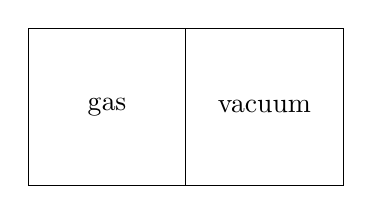
\begin{tikzpicture}
      \draw (0, 0) rectangle (4, 2);
      \draw (2, 0) -- (2, 2);
      \node at (1, 1) {gas};
      \node at (3, 1) {vacuum};
    \end{tikzpicture}
  \end{center}
  We have a valve in the partition, and as soon as we open up the valve, the gas flows to the other side of the box.

  In this system, no energy has been supplied. So $\d E = 0$. However, $\d V > 0$, as volume clearly increased. But there is no work done on or by the gas. So in this case, $-p \;\d V$ is certainly not the work done. Using the first law, we know that
  \[
    T \;\d S = p \;\d V.
  \]
  So as the volume increases, the entropy increases as well.
\end{eg}

We now revisit the concept of heat capacity. We previously defined it as $\d E/\d T$, but now we need to decide what we want to keep fixed. We can keep $V$ fixed, and get
\[
  C_V = \left(\frac{\partial E}{\partial T}\right)_V = T \left(\frac{\partial S}{\partial T}\right)_V.
\]
While this is the obvious generalization of what we previously had, it is not a very useful quantity. We do not usually do experiments with fixed volume. For example, if we do a chemistry experiment in a test tube, say, then the volume is not fixed, as the gas in the test tube is free to go around. Instead, what is fixed is the pressure. We can analogously define
\[
  C_p = T \left(\frac{\partial S}{\partial T}\right)_p.
\]
Note that we cannot write this as some sort of $\frac{\partial E}{\partial T}$.

\subsection{The canonical ensemble}
So far, we have been using the microcanonical ensemble. This is a system with the energy known. This is appropriate for an isolated system, where the energy cannot change.

However, most systems are \emph{not} isolated, eg. a glass of water in the room. What \emph{is} fixed is the temperature. The \emph{canonical ensemble} describes exactly that --- we know the temperature, but not energy.

Imagine we have a system $S$, and it is interacting with a much larger system $R$. We call this $R$ a \emph{heat reservoir}. Since $R$ is assumed to be large, the energy of $S$ is negligible to $R$, and we will assume $R$ always has a fixed temperature $T$. Then in this set up, the system can exchange energy without changing $T$.

As before, we let $\bket{n}$ be a basis of microstates with energy $E_n$. We suppose we fix a total energy $E_{\mathrm{total}}$, and we want to find the total number of microstates of the combined system with this total energy. To do so, we fix some state $\bket{n}$ of $S$, and ask how many states of $S + R$ there are for which $S$ is in $\bket{n}$. We then later sum over all $\bket{n}$.

By definition, we can write this as
\[
  \Omega_R(E_{\mathrm{total}} - E_n) = \exp\left(k^{-1} S_R(E_{\mathrm{total}} - E_n)\right).
\]
Since $R$ is assumed to be much larger than $E$, we only get sensible contributions

By assumption, we know $R$ is a much larger system than $S$. So we only get significant contributions when $E_n \ll E_{\mathrm{total}}$. In these cases, we can Taylor expand to write
\[
  \Omega_R(E_{\mathrm{total}} - E_n) = \exp\left(k^{-1} S_R(E_{\mathrm{total}}) - \left(\frac{\partial S}{\partial E}\right)_V E_n\right).
\]
But we know what $\frac{\partial S_R}{\partial E}$ is --- it is just $T^{-1}$. So we finally get
\[
  \Omega_R(E_{\mathrm{total}} - E_n) = e^{k^{-1}S_R(E_{\mathrm{total}})} e^{-\beta E_n},
\]
where we define
\begin{defi}[$\beta$]\index{$\beta$}
  \[
    \beta = \frac{1}{kT}.
  \]
\end{defi}
Note that while we derived this this formula under the assumption that $E_n$ is small, it is effectively still valid when $E_n$ is large, because both sides are very tiny, and even if they are very tiny in different ways, it doesn't matter when we add over all states.

Now we can write the \emph{total} number of microstates of $S + R$ as
\[
  \Omega(E_{\mathrm{total}}) = \sum_n \Omega_R(E_{\mathrm{total}} - E_n) = e^{k^{-1} S_R(E_{\mathrm{total}})} \sum_n e^{-\beta E_n}.
\]
Note that we are summing over all states, not energy.

We now use the fundamental assumption of statistical mechanics that all states of $S + R$ are equally likely. Then we know the probability that $S$ is in state $\bket{n}$ is
\[
  p(n) =\frac{\Omega_R(E_{\mathrm{total}} - E_n)}{\Omega(E_{\mathrm{total}})} = \frac{e^{-\beta E_n}}{\sum_k e^{-\beta E_k}}.
\]
This is called the \term{Boltzmann distribution} for the canonical ensemble. Note that at the end, all the details have dropped out apart form the temperature. This describes the energy distribution of a system with fixed temperature.

Note that if $E_n \gg kT = \frac{1}{\beta}$, then the exponential is small. So only states with $E_n \sim kT$ have significant probability. In particular, as $T \to 0$, we have $\beta \to \infty$, and so only the ground state can be occupied.

We now define an important quantity.
\begin{defi}[Partition function]\index{partition function}
  The \emph{partition function} is
  \[
    Z = \sum_n e^{-\beta E_n}.
  \]
\end{defi}
So we have
\[
  p(n) = \frac{e^{-\beta E_n}}{Z}.
\]
\begin{prop}
  For two non-interacting systems, we have $Z(\beta) = Z_1(\beta) Z_2(\beta)$.
\end{prop}

\begin{proof}
  Since the systems are not interacting, we have
  \[
    Z = \sum_{n, m} e^{-\beta (E_n^{(1)} + E_n^{(2)})} = \left(\sum_n e^{-\beta E_n^{(1)}}\right)\left(\sum_n e^{-\beta E_n^{(2)}}\right) = Z_1 Z_2.
  \]
\end{proof}

Note that in general, energy is \emph{not} fixed, but we can compute the average value:
\[
  \bra E\ket = \sum_n p(n) E_n = \sum \frac{E_n e^{-\beta E_n}}{Z} = -\frac{\partial}{\partial \beta} \log Z.
\]
This partial derivative is taken with all $E_i$ fixed. Of course, in the real world, we don't get to directly change the energy eigenstates and see what happens. However, they do depend on some ``external'' parameters, such as the volume $V$, the magnetic field $B$ etc. So when we take this derivative, we have to keep all those parameters fixed.

We look at the simple case where $V$ is the only parameter we can vary. Then $Z = Z(\beta, V)$. We can rewrite the previous formula as
\[
  \bra E \ket = - \left(\frac{\partial}{\partial \beta} \log Z\right)_V.
\]
This gives us the average, but we also want to know the variance of $E$. We have
\[
  \Delta E^2 = \bra (E - \bra E\ket)^2 \ket = \bra E^2\ket - \bra E\ket^2.
\]
On the first example sheet, we calculate that this is in fact
\[
  \Delta E^2 = \left(\frac{\partial^2}{\partial \beta^2} \log Z\right)_V = - \left(\frac{\partial \bra E\ket}{\partial \beta}\right)_V.
\]
We can now convert $\beta$-derivatives to $T$-derivatives using the chain rule. Then we get
\[
  \Delta E^2 = kT^2 \left(\frac{\partial \bra E\ket}{\partial T}\right)_V = kT^2 C_V.
\]
So the fluctuation around the expectation is actually proportional to the heat capacity.

From this, we can learn something important. We would expect $\bra E\ket \sim N$, the number of particles of the system. But we also know $C_V \sim N$. So
\[
  \frac{\Delta E}{\bra E\ket} \sim \frac{1}{\sqrt{N}}.
\]
Therefore, the fluctuations are negligible if $N$ is large enough. This is called the \term{thermodynamic limit} $N \to \infty$. In this limit, we can ignore the fluctuations in energy. So we expect the microcanonical ensemble and the canonical ensemble to give the same result. And for all practical purposes, $N \sim 10^{23}$ is a large number.

Because of that, we are often going to just write $E$ instead of $\bra E\ket$.

\begin{eg}
  Suppose we had particles with
  \[
    E_{\uparrow} = \varepsilon,\quad E_{\downarrow} = 0.
  \]
  So for one particle, we have
  \[
    Z_1 = \sum_n e^{-\beta E_n} = 1 + e^{-\beta \varepsilon} = 2 e^{-\beta \varepsilon/2} \cosh \frac{\beta \varepsilon}{2}.
  \]
  If we have $N$ non-interacting systems, then since the partition function is multiplicative, we have
  \[
    Z = Z_1^N = 2^n e^{-\beta \varepsilon N/2} \cosh^N \frac{\beta \varepsilon}{2}.
  \]
  From the partition function, we can compute
  \[
    \bra E \ket = - \frac{\d \log Z}{\d \beta} = \frac{N\varepsilon}{2}\left(1 - \tanh \frac{\beta \varepsilon}{2}\right).
  \]
  We can check that this agrees with the value we computed with the microcanonical ensemble (when we wrote the result using exponentials directly), but the calculation is much easier.
\end{eg}

\subsubsection*{Entropy}
We now want to talk about the entropy of the canonical ensemble, but we do not really have a working definition for it, as the Boltzmann definition only applies to the microcanonical ensemble. So we need a new definition.

We can motivate our new definition as follows --- recall that we can think of the ensemble as having $W \gg 1$ copies of the world with $Wp(n)$ copies in the state $\bket{n}$. We now try to apply the Boltzmann definition of entropy
\[
  S = k \log \Omega
\]
to the whole ensemble, where now $\Omega$ is the number of ways of choosing which copy is in which state. This is just
\[
  \Omega = \frac{W!}{\prod_n (W p(n))!}.
\]
We can use Stirling's approximation, and find that
\[
  S_{\mathrm{ensemble}} = -kW \sum_n p(n) \log p(n).
\]
This suggests that we should define the entropy of a single copy as follows:
\begin{defi}[Gibbs entropy]\index{Gibbs entropy}
  The \emph{Gibbs entropy} of a probability distribution $p(n)$ is
  \[
    S = -k \sum_n p(n) \log p(n).
  \]
\end{defi}
If the density operator is given by
\[
  \hat{\rho} = \sum_n p(n) \bket{n}\brak{n},
\]
then we have
\[
  S = - \Tr(\hat{\rho} \log \hat{\rho}).
\]
We now check that this definition makes sense, in that when we have a microcanonical ensemble, we do get what we expect.
\begin{eg}
  In the microcanonical ensemble, we have
  \[
    p(n) =
    \begin{cases}
      \frac{1}{\Omega(E)} & E \leq E_n \leq E + \delta E\\
      0 & \text{otherwise}
    \end{cases}
  \]
  Then we have
  \[
    S = -k \sum_{n: E \leq E_n \leq E + \delta E} \frac{1}{\Omega(E)} \log \frac{1}{\Omega(E)} = -k \Omega(E) \frac{1}{\Omega(E)} \log \frac{1}{\Omega(E)} = k \log \Omega(E).
  \]
  So the Gibbs entropy reduces to the Boltzmann entropy.
\end{eg}

How about the canonical ensemble?
\begin{eg}
  In the canonical ensemble, we have
  \[
    p(n) = \frac{e^{-\beta E_n}}{Z}.
  \]
  Plugging this into the definition, we find that
  \begin{align*}
    S &= -k \sum_n p(n) \log \left(\frac{e^{-\beta E_n}}{Z}\right)\\
    &= -k \sum_n p(n) (-\beta E_n - \log Z)\\
    &= k \beta \bra E\ket + k\log Z,
  \end{align*}
  using the fact that $\sum p(n) = 1$.

  Using the formula of the expected energy, we find that this is in fact
  \[
    S = k \frac{\partial}{\partial T} (T \log Z)_V.
  \]
\end{eg}

\subsubsection*{Maximizing entropy}
It turns out we can reach the canonical ensemble in a different way. The second law of thermodynamics suggests we should always seek to maximize entropy. Now if we take the optimization problem of ``maximizing entropy'', what probability distribution will we end up with?

The answer depends on what constraints we put on the optimization problem. We can try to maximize $S_{\mathrm{Gibbs}}$ over all probability distributions such that $p(n) = 0$ unless $E \leq E_n \leq E + \delta E$. Of course, we also have the constraint $\sum p(n) = 1$. Then we can use a Lagrange multiplier $\alpha$ and extremize
\[
  k^{-1}S_{\mathrm{Gibbs}} + \alpha \left(\sum_n p(n) - 1\right),
\]
Differentiating with respect to $p(n)$ and solving, we get
\[
  p(n) = e^{\alpha - 1}.
\]
In particular, this is independent of $n$. So all microstates with energy in this range are equally likely, and this gives the microcanonical ensemble.

What about the canonical ensemble? It turns out this is obtained by maximizing the entropy over all $p(n)$ such that $\bra E\ket$ is fixed. The computation is on the first example sheet.

\subsection{Helmholtz free energy}

In the microcanonical ensemble, we discussed the second law of thermodynamics, namely the entropy increases with time and the maximum is achieved in an equilibrium.

But this is no longer true in the case of the canonical ensemble, because we now want to maximize the total entropy of the system plus the heat bath, instead of just the system itself. Then is there a proper analogous quantity for the canonical ensemble?

The answer is given by the \emph{free energy}. In the canonical ensemble, the probability of energy being between $E$ and $E + \delta E$ (for $\delta E \ll kT$) is given by
\[
  p(E) = \Omega_S(E) \frac{e^{-\beta E}}{Z} = \frac{1}{Z} e^{k^{-1} S - \beta E} = \frac{1}{Z} e^{-\beta (E - TS)}
\]
where $\Omega_S(E)$ is the number of states with energy between $E$ and $\delta E$. Here we assumed that $\delta E$ is small so that the probabilities of the different particles are similar. % fix this

We define
\begin{defi}[Helmholtz free energy]\index{Helmholtz free energy}\index{free energy!Helmholtz}
  The \emph{Helmholtz free energy} is
  \[
    F = E - TS,
  \]
\end{defi}
Then we have
\[
  p(E) = \frac{1}{Z} e^{-\beta F}.
\]
So in the canonical ensemble, the most likely $E$ is the one that minimizes $F$.

In general, in an isolated system, $S$ increases, and $S$ is maximized in equilibrium. In a system with a reservoir, $F$ decreases, and $F$ minimizes in equilibrium. In some sense $F$ captures the competition between entropy and energy. We will discuss this further later.

Now is there anything analogous to the first law
\[
  \d E = T \d S - p \d V?
\]
Since we have $S$ and $V$ on the right, here we are regarding energy as a function of entropy and volume, or entropy as a function of $E$ and $V$. Using this, we can write
\[
  \d F = \d E - \d(TS) = -S \d T - p \d V.
\]
So it is natural to think of $F$ as a function of $T$ and $V$. Mathematically, the relation between $F$ and $E$ is that $F$ is the \term{Legendre transform} of $E$.

From this expression, we can immediately write down
\[
  S = - \left(\frac{\partial F}{\partial T}\right)_V,
\]
and the pressure is
\[
  p = -\left(\frac{\partial F}{\partial V}\right)_T.
\]
The final claim about the free energy is that we have a very useful formula for it.
\begin{prop}
  \[
    F = -kT \log Z.
  \]
  Alternatively,
  \[
    Z = e^{-\beta F}.
  \]
\end{prop}

\begin{proof}
  We use the fact that
  \[
    \frac{\d}{\d \beta} = kT^2 \frac{\d}{\d T}.
  \]
  Then we can start from
  \begin{align*}
    F &= E - TS \\
    &= - \left(\frac{\partial \log Z}{\partial \beta}\right) - TS \\
    &= kT^2 \left(\frac{\partial \log Z}{\partial T}\right)_V - kT \frac{\partial}{\partial T}(T \log Z)_V\\
    &= -k T \log Z,
  \end{align*}
  and we are done. Good.
\end{proof}

\subsection{The chemical potential}
So far we have considered situations where we had fixed energy or fixed volume. However, there are often other things that are fixed. For example, the number of particles, or the electric charge of the system would be fixed. If we measure these things, then this restricts which microstates are accessible.

Let's consider $N$. This quantity was held fixed in the microcanonical and canonical ensembles. But these quantities do depend on $N$, and we can write
\[
  S(E, V, N) = k \log \Omega(E, V, N).
\]
Previously, we took this expression, and asked what happens when we varied $E$, and we got temperature. We then asked what happens when we vary $V$, and we got pressure. Now we ask what happens when we vary $N$.
\begin{defi}[Chemical potential]\index{chemical potential}
  The \emph{chemical potential} of a system is given by
  \[
    \mu = -T \left(\frac{\partial S}{\partial N}\right)_{E, V}.
  \]
\end{defi}

Why is this significant? Recall that when we only varied $E$, then we figured that two systems in equilibrium must have equal temperature. Then we varied $V$ as well, and found that two systems in equilibrium must have equal temperature \emph{and} pressure. Then it shouldn't be surprising that if we have two interacting systems that can exchange particles, then we must have equal temperature, pressure \emph{and} chemical potential. Indeed, the same argument works.

If we want to consider what happens to the first law when we vary $N$, we can just straightforwardly write
\[
  \d S = \left(\frac{\partial S}{\partial E}\right)_{V, N} \d E + \left(\frac{\partial S}{\partial V}\right)_{E, N} \d V + \left(\frac{\partial S}{\partial N}\right)_{E, V} \d V.
\]
Then as before, we get
\[
  \d E = T \;\d S - p \;\d V + \mu \;\d N.
\]
From this expressions, we can get some feel for what $\mu$ is. This is the energy cost of adding one particle at $S, V$. We will actually see later that $\mu$ is actually negative, as it is hard to add a particle keeping the entropy fixed.

Note that if we change $N$ to $Q$, then $\mu$ changes into $\Phi$, the electrostatic potential.

From the first law, we can write
\[
  \mu = \left(\frac{\partial E}{\partial N}\right)_{S, V}.
\]
We might ask, can we obtain this result from the original definition directly? Indeed, we can, using the magic identity
\[
  \left(\frac{\partial x}{\partial y}\right)_z \left(\frac{\partial y}{\partial z}\right)_x \left(\frac{\partial z}{\partial x}\right)_y = -1.
\]
In the canonical ensemble, we have fixed $T$, but the free energy will also depend on energy:
\[
  F(T, V, N) = E - TS.
\]
Again, we have
\[
  \d F = \d E - \d (TS) = -S\;\d T - p\;\d V + \mu\;\d N.
\]
So we have
\[
  \mu = \left(\frac{\partial F}{\partial N}\right)_{T, V}.
\]
\subsection{Grand canonical ensemble}
Consider a system $S$ in equilibrium with a ``heat and particle'' reservoir $R$, with which it can exchange both heat and particles. Again, $\mu$ and $T$ are fixed by their values in $R$. We repeat the argument with the canonical ensemble, and we will find that the probability that a system is in state $n$ is
\[
  p(n) = \frac{e^{-\beta (E_n - \mu N_n)}}{\mathcal{Z}},
\]
where $N_n$ is the number of particles in $\bket{n}$, and
\[
  \mathcal{Z} = \sum_n e^{-\beta(E_n- \mu N_n)}
\]
is the \term{grand canonical partition function}.

Of course, we can introduce more and more quantities after $V, N$, and then get more and more terms in the partition function, but they are really just the same. We can quickly work out how we can compute quantities from $Z$. By writing out the expressions, we have
\begin{prop}
  \[
    \bra E \ket - \mu \bra N\ket = -\left(\frac{\partial \mathcal{Z}}{\partial \beta}\right)_{\mu, V}.
  \]
\end{prop}

\begin{prop}
  \[
    \bra N\ket = \sum_n p(n) N_n = \frac{1}{\beta} \left(\frac{\partial \log \mathcal{Z}}{\partial \mu}\right)_{T, V}.
  \]
\end{prop}

As in the canonical ensemble, there is a simple formula for variance:
\begin{prop}
  \[
    \nabla N^2 = \bra N^2 \ket - \bra N\ket^2 = \frac{1}{\beta^2} \left(\frac{\partial^2 \log Z}{\partial \mu^2}\right)_{T, V} = \frac{1}{\beta} \left(\frac{\partial \bra N\ket}{\partial \mu}\right)_{T, V} \sim N.
  \]
  So we have
  \[
    \frac{\Delta N}{ \bra N\ket} \sim \frac{1}{\sqrt{N}}.
  \]
\end{prop}

So again in the thermodynamic limit, the fluctuations in $\bra N\ket$ are negligible.

We can also calculate the Gibbs entropy:
\begin{prop}
  \[
    S = k \beta (\bra E \ket - \mu \bra N\ket) + k \log \mathcal{Z} - k \beta \left(\frac{\partial \log \mathcal{Z}}{\partial \beta}\right)_{\mu, V} + k \log \mathcal{Z} = k \frac{\partial}{\partial T}(T \log \mathcal{Z})_{\mu, N}.
  \]
\end{prop}

With the canonical ensemble, we had the free energy. There is an analogous thing we can define for the grand canonical ensemble.
\begin{defi}[Grand canonical potential]\index{grand canonical potential}\index{$\Phi$}
  The \emph{Grand canonical potential} is
  \[
    \Phi = F - \mu N = E - TS - \mu N.
  \]
\end{defi}
Then we have
\begin{prop}
  \[
    \d \Phi = - S \;\d T - p \;\d V - N \;\d \mu.
  \]
\end{prop}
We thus see that it is natural to view $\Phi$ as a function of $T$, $V$ and $\mu$. Using the formula for $E - \mu N$, we find
\[
  \Phi = - \left(\frac{\partial \log \mathcal{Z}}{ \partial \beta}\right)_{\mu, V} = - kT \frac{\partial}{\partial T} (\log \mathcal{Z})_{\mu, V} = -kT \log \mathcal{Z},
\]
which is exactly the form we had for the free energy in the canonical ensemble. In particular, we have
\[
  \mathcal{Z} = e^{-\beta \Phi}.
\]
\subsection{Extensive and intensive properties}
The quantities we separate into two different types. There are things like $V, N$ etc that scale with the size of the volume. On the other hand, we have things like $\mu$ and $p$ do not scale with the size.

\begin{defi}[Extensive quantity]\index{extensive quantity}
  An \emph{extensive quantity} is one that scales proportionally to the size of the system
\end{defi}

\begin{eg}
  $N, V, E, S$ are all extensive quantities.
\end{eg}

Now note that the entropy is a function of $E, V, N$. So if we scale a system by $\lambda$, we find that
\[
  S(\lambda E, \lambda V, \lambda N) = \lambda S(E, V, N).
\]
\begin{defi}[Intensive quantity]\index{intensive quantity}
  An \emph{intensive quantity} is one that is independent of the size of the system.
\end{defi}

\begin{eg}
  Recall that we defined
  \[
    \frac{1}{T} = \left(\frac{\partial S}{\partial E}\right))_{V, N}.
  \]
  So if we scale the system by $\lambda$, then both $S$ and $E$ scale by $\lambda$, and so $T$ does not change. Similarly,
  \[
    p = T \left(\frac{\partial S}{\partial V}\right)_{T, N},\quad \mu = -T \left(\frac{\partial S}{\partial N}\right)_{T, V}
  \]
  are intensive quantities.
\end{eg}

\begin{eg}
  The \emph{free energy} is defined by
  \[
    F = E - TS.
  \]
  Since $E$ and $S$ are both extensive, and $T$ is intensive, we find that $F$ is extensive. So
  \[
    F (T, \lambda V, \lambda N) = \lambda F(T, V, N).
  \]
  Similarly, the grand canonical potential is
  \[
    \Phi = F - \mu N.
  \]
  Since $F$ and $N$ are extensive and $\mu$ are intensive, we know $\Phi$ is extensive:
  \[
    \Phi(T, \lambda V, \mu) = \lambda \Phi(T, V, \mu).
  \]
\end{eg}
This tells us something useful. We see that $\Phi$ must be proportional to $V$. Indeed, taking the above equation with respect to $\lambda$< we find
\[
  V \left(\frac{\partial \Phi}{\partial V}\right)_{T, \mu} (T, \lambda V, \mu) = \Phi(T, V, \mu).
\]
Now setting $\lambda = 1$, we find
\[
  \Phi(T, V, \mu) = V \left(\frac{\partial \Phi}{\partial V} \right)_{T, \mu} = -pV.
\]
Here $p$ is an intensive quantity, it cannot depend on $V$. So we have
\[
  \Phi(T, V, \mu) = -p(T, \mu) V.
\]
This is quite a strong result.

\section{Classical gases}
So far, we have been doing statistical physics starting from quantum mechanics. But statistical mechanics was invented \emph{before} quantum mechanics. So we should be able to do statistical mechanics classically, and we will apply it to the case of classical gases. This classical theory agree quite well with experiment, except for a few small things that went wrong, and it turns out we have to solve these problems by going quantum.

To do statistical physics classically, the idea is to figure out what the classical version of the partition function should be. We can then use this to derive the different thermodynamic quantities, as we have previously managed to express them in terms of the partition function.

After figuring out the partition function, we are going to study three types of classical gases. We begin by looking at monoatomic ideal gases, which is the simplest type of gases one can think of. They do not have internal structure and do not interact with each other.

After understanding monoatomic ideal gases, we will move on to consider two possible modifications. The first is the case of a diatomic (ideal) gas, where the gases now have some internal structure, and hence kinetic energy is not the only possible kind of energy. It turns out the theory works out pretty similarly to the monoatomic case, except that the average energy of each particle is higher than the ideal gas version.

Finally, we will consider what happens if we have gas molecules that do interact with each other, and we will do so perturbatively, assuming the interactions are small (which they are).

\subsection{The classical partition function}
In the canonical ensemble, the quantum partition function is
\[
  Z = \sum_n e^{-\beta E_n}.
\]
What is the classical analogue? Classically, we can specify the state of a system by a point in \term{phase space}, which is the space of all positions and momentum.

For example, if we have a simple particle, then a point in phase space is just $(\mathbf{q}(t), \mathbf{p}(t))$, the position and momentum of the particle. It is conventional to use $\mathbf{q}$ instead of $\mathbf{x}$ when talking about a point in the phase space. So in this case, the phase space is a $6$-dimensional space.

The equation of motion determines the trajectory of the particle through phase space, given the initial position in phase space. This suggests that we should replace the sum over states by an integral over phase space. Classically, we also know what the energy is. For a single particle, the energy is given by the Hamiltonian
\[
  H = \frac{\mathbf{p}^2}{2m} + V(\mathbf{q}).
\]
So it seems that we know what we need to know to make sense of the partition function classically. We might want to define the partition function as
\[
  Z_1 = \int \d^3 q\; \d^3 p\; e^{-\beta H(\mathbf{p}, \mathbf{q})}.
\]
This seems to make sense, except that we expect the partition function to be dimensionless. The solution is to introduce a quantity $h$, which has dimensions of length times momentum. Then we have
\begin{defi}[Partition function (single particle)]\index{partition function!single particle}
  We define the \emph{single particle partition function} as
  \[
    Z_1 = \frac{1}{h^3} \int \d^3 q\; \d^3 p\; e^{-\beta H(\mathbf{p}, \mathbf{q})}.
  \]
\end{defi}
We notice that whenever we use the partition function, we usually differentiate the log of $Z$. So the factor of $h^3$ doesn't really matter for observable quantities.

However, recall that entropy is just given by $\log Z$, and we might worry that the entropy depends on $Z$. But it doesn't matter, because entropy is not actually observable. Only entropy differences are. So we are fine.

The more careful reading might worry that our choice to integrate $e^{-\beta H(\mathbf{p}, \mathbf{q})}$ against $\d^3 q\; \d^e p$ is rather arbitrary, and there is no good \emph{a priori} reason why we shouldn't integrate it against, say, $\d^3 q\; \d^3 p^5$ instead.

However, it is possible to show that this is indeed the ``correct'' partition function to use, by taking the quantum partition function, and then taking the limit $\hbar \to 0$. Moreover, we find that the correct value of $h$ should be
\[
  h = 2\pi \hbar.
\]
We will from now on use this value of $h$.

\subsection{Monoatomic ideal gas}
We now begin considering ideal gases.
\begin{defi}[Ideal gas]\index{ideal gas}
  An \emph{ideal gas} is a gas where the particles do not interact with each other.
\end{defi}
Of course, this is never true, but we can hope this is a good approximation when the particles are far apart.

We begin by considering a \term{monoatomic ideal gas}\index{ideal gas!monoatomic}. These gases have no internal structure, and is made up of single atoms. In this case, the only energy we have is the kinetic energy, and we get
\[
  H = \frac{\mathbf{p}^2}{2m}.
\]
We just have to plug this into our partition function and evaluate the integral. We have
\begin{align*}
  Z_1(V, T) &= \frac{1}{(2\pi \hbar)^3} \int \d^3 p\; \d^3 q\; e^{-\beta \mathbf{p}^2 /2m}\\
  &= \frac{V}{(2\pi \hbar)^3} \int \d^3 p\; e^{-\beta \mathbf{p}^2/2m}
\end{align*}
Here $V$ is the volume of the box containing the particle, which is what we obtain when we do the $\d^3 q$ integral.

This remaining integral is just the Gaussian integral. Recall that we have
\[
  \int \d x\; e^{-a x^2} = \sqrt{\frac{\pi}{a}}.
\]
Using this three times, we find
\begin{prop}
  For a monoatomic gas, we have
  \[
    Z_1(V, T) = V\left(\frac{mkT}{2\pi \hbar^2}\right)^{3/2} = \frac{V}{\lambda^3},
  \]
\end{prop}
where we define
\begin{defi}[Thermal de Broglie wavelength]\index{thermal de Broglie wavelength}\index{$\lambda$}\index{de Broglie wavelength!thermal}
  The \emph{thermal de Broglie wavelength} of a gas at temperature $T$ is
  \[
    \lambda = \sqrt{\frac{2\pi \hbar^2}{mkT}}.
  \]
\end{defi}
If we think of the wavelength as the ``size'' of the particle, then we see that the partition function counts the number of particles we can fit in the volume $V$. We notice that this partition function involves $\hbar$, which is a bit weird since we are working classically, but we will see that the $\hbar$ doesn't appear in the formulas we derive from this.

The generalization to multiple particles is straightforward. If we have $N$ particles, since the partition function is again multiplicative, we have
\[
  Z(N, V, T) = Z_1^N = V^N \lambda^{-3N}.
\]
There is a small caveat at this point. We will later see that this is not quite right. When we think about the quantum version, if the particles are indistinguishable, then we would have counted each state $N!$ times, which would give the wrong answer. Again, this doesn't affect any observable quantity, so we will put this issue aside for the moment, until we get to studying the entropy itself, in which case this $N!$ \emph{does} matter.

We can similarly \emph{define} the pressure to be
\[
  p = - \left(\frac{\partial F}{\partial V}\right)_T = \frac{\partial}{\partial V} (k T \log Z)_T.
\]
Then plugging our partition function into this definition, we find
\[
  p = \frac{NkT}{V}.
\]
Rearranging, we obtain
\begin{prop}[Ideal gas law]\index{ideal gas law}
  \[
    pV = NkT.
  \]
\end{prop}
Notice that in this formula, the $\lambda$ has dropped out, and there is no dependence on $\hbar$. Such an equation is known as an \emph{equation of state}.

\begin{defi}[Equation of state]\index{equation of state}
  An \emph{equation of state} is an equation that relates state variables, ie. variables that depend only on the current state of the system, as opposed to how we obtained to this system.
\end{defi}

Let's now look at the energy of the ideal gas. We can similarly compute
\[
  \bra E\ket = - \left(\frac{\partial \log Z}{\partial \beta}\right)_V = \frac{3}{2} NkT = 3N \left(\frac{1}{2} kT\right).
\]
This is a general phenomenon. Our system has $N$ particles, and each particle has three independent directions it can move in. So there are $3N$ degrees of freedom.
\begin{law}[Equipartition of energy]\index{Equipartition of energy}
  Each degree of freedom of an ideal gas contributes $\frac{1}{2}kT$ to the average energy.
\end{law}
In the next section, we will study gases with internal structure, hence internal degrees of freedom, and each such degree of freedom will again contribute $\frac{1}{2}kT$ to the average energy.

Of course, this law requires some hidden assumptions we do not make precise. If we add a degree of freedom $s$ with a term $s^{5.3} \log (2s + 1)$ in the Hamiltonian, then there is no reason to believe the contribution to the average energy would again be $\frac{1}{2} kT$. We will also see in the next section that if the degree of freedom has some potential energy, then there will be even more contribution to the energy.

There are other quantities of the gas we can compute. We know the average energy of a single particle is
\[
  \frac{\bra \mathbf{p}^2\ket}{2m} = \frac{3}{2} kT.
\]
So we have
\[
  \bra \mathbf{p}^2 \ket \sim mkT.
\]
Thus, for a single particle, we have
\[
  |\mathbf{p}| \sim \sqrt{mKt},
\]
and so
\[
  \lambda \sim \frac{h}{|\mathbf{p}|}.
\]
This is the usual formula for the de Broglie wavelength. So our thermal de Broglie wavelength is indeed related to the de Broglie wavelength.

Finally, we can compute the heat capacity
\[
  C_V = \left(\frac{\partial E}{\partial T}\right)_V = \frac{3}{2}Nk.
\]
\subsubsection*{Boltzmann's constant}
Recall that Boltzmann's constant is
\[
  k = \SI{1.381e-23}{\joule\per\kelvin}
\]
This number shows that we were terrible at choosing units. If we were to invent physics again, we would pick energy to have the same unit as temperature, so that $k = 1$. This number $k$ is just a conversion factor between temperature and energy because we chose the wrong units.

But of course, the units were not chosen randomly in order to mess up our thermodynamics. The units were chosen to relate to scales we meet in everyday life. So it is still reasonable to ask why $k$ has such a small value. We look at the ideal gas law.
\[
  \frac{pV}{T} = Nk.
\]
We would expect when we plug in some everyday values for the left hand side, the result would be somewhat sensible, because our ancestors were sane when picking units (hopefully).

Indeed, we can put in numbers
\begin{align*}
  p &= \SI{e5}{\newton\per\meter\squared}\\
  V &= \SI{1}{\meter\cubed}\\
  T &= \SI{300}{\kelvin},
\end{align*}
and we find that the LHS is $\sim 300$.

So what makes $k$ such a tiny number is that $N$ is huge. The number of particles is of the order $10^{23}$. Thus, for $Nk$ to have a sensible value, $k$ must be tiny.

The fact that $k$ is small tells us that everyday lumps of matter contain a lot of particles, and in turn, this tells us that atoms are small.

\subsubsection*{Entropy}
The next thing to study is the entropy of an ideal gas. We previously wrote down
\[
  Z = Z_1^N,
\]
and briefly noted that this isn't actually right. In quantum mechanics, we know that if we swap two indistinguishable particles, then we get back the same state, at least up to a sign. Similarly, if we permute any of our particles, which are indistinguishable, then we get the same system. We are over-counting the states. What we really should do is to divide by the number of ways to permute the particles, namely $N!$:
\[
  Z = \frac{1}{N!} Z_1^N.
\]
Just as in the constant $h$ in our partition function, this $N!$ doesn't affect any of our observables. In particular, $p$ and $\bra E\ket$ are unchanged. However, this $N!$ does affect the entropy
\[
  S = \frac{\partial}{\partial T} (kT \log Z).
\]
Plugging the partition function in and using Stirling's formula, we get
\[
  S = Nk \left(\log \left(\frac{V}{N\lambda^3}\right) + \frac{5}{2}\right).
\]
This is known as the \term{Sackur-Tetrode equation}.

Recall that the entropy is an extensive property. If we re-scale the system by a factor of $\alpha$, then
\[
  N \mapsto \alpha N,\quad V \mapsto \alpha V.
\]
Since $\lambda$ depends on $T$ only, it is an intensive quantity, and this indeed scales as $S \mapsto \alpha S$. But for this to work, we really needed the $N$ inside the logarithm, and the reason we have the $N$ inside the logarithm is that we had an $N!$ in the partition function.

When people first studied statistical mechanics of ideal gases, they didn't know about quantum mechanics, and didn't know they should put in the $N!$. Then the resulting value of $S$ is no longer extensive. This leads to \term{Gibbs paradox}. The actual paradox is as follows:

Suppose we have a box of bas with entropy $S$. We introduce a partition between the gases, so that the individual partitions have entropy $S_1$ and $S_2$. Then the fact that the gas is not extensive means
\[
  S \not= S_1 + S_2.
\]
This means by introducing or removing a partition, we have increased or decreased the entropy, which violates the second law of thermodynamics.

This $N!$, which comes from quantum effects, fixes this problem. This is a case where quantum mechanics is needed to understand something that really should be classical.

\subsubsection*{Grand canonical ensemble}
We now consider the case where we have a grand canonical ensemble, so that we can exchange heat \emph{and} particles. In the case of gas, we can easily visualize this as a small open box of gas where gas is allowed to freely flow around. The grand ensemble has partition function
\begin{align*}
  \mathcal{Z}_{\mathrm{ideal}}(\mu, V, T) &= \sum_{N = 0}^\infty e^{\beta \mu N} Z_{\mathrm{ideal}}(N, V, T) \\
  &= \sum_{N = 0}^\infty \frac{1}{N!} \left(\frac{e^{\beta \mu} V}{\lambda^3}\right)^N\\
  &= \exp\left(\frac{e^{\beta \mu}V}{\lambda^3}\right)
\end{align*}
Armed with this, we can now calculate the average number of particles in our system. Doing the same computations as before, we have
\[
  N = \frac{1}{\beta} \left(\frac{\partial \log Z}{\partial \mu}\right)_{V, T} = \frac{e^{\beta \mu}V}{\lambda^3}.
\]
So we can work out the value of $\mu$:
\[
  \mu = kT \log \left(\frac{\lambda^3 N}{V}\right).
\]
Now we can use this to get some idea of what the chemical potential actually means. For a classical gas, we need the wavelength to be significantly less than the average distance between particles, ie.
\[
  \lambda \ll \left(\frac{V}{N}\right)^{1/3},
\]
so that the particles are sufficiently separated. If this is not true, then quantum effects are important, and we will look at them later. If we plug this into the logarithm, we find that $\mu < 0$.

Remember that $\mu$ is defined by
\[
  \mu = \left(\frac{\partial E}{\partial N}\right)_{S, V}.
\]
It might seem odd that we get energy out when we add a particle. But note that this derivative is taken with $S$ fixed. Normally, we would expect adding a particle to increase the entropy. So to keep the entropy fixed, we must simultaneously take out energy of the system, and so $\mu$ is negative.

Continuing our exploration of the grand canonical ensemble, we can look at the fluctuations in $N$, and find
\[
  \Delta N^2 = \frac{1}{\beta^2} \log \mathcal{Z}_{\mathrm{ideal}} = N.
\]
So we find that
\[
  \frac{\Delta N}{N} = \frac{1}{\sqrt{N}} \to 0
\]
as $N \to \infty$. So in the thermodynamic limit, the fluctuations are negligible.

We can now obtain our equation of state. Recall the grand canonical potential is
\[
  \Phi = -kT \log \mathcal{Z},
\]
and that
\[
  pV = -\Phi.
\]
Since we know $\log \mathcal{Z}$, we can work out what $pV$ is, we find that
\[
  pV = kT \frac{e^{\beta \mu}V}{\lambda^3} = NkT.
\]
So the ideal gas law\index{ideal gas law} is also true in the grand canonical ensemble. Also, from cancelling the $V$ from both sides, we see that this determines $p$ as a function of $T$ and $\mu$:
\[
  p = \frac{kT e^{\beta\mu}}{\lambda^3}.
\]

\subsection{Maxwell distribution}
We calculated somewhere the average energy of our gas, so we can calculate the average energy of an atom in the gas. But that is just the average energy. We might want to figure out the distribution of energy in the atoms of our gas. Alternatively, what is the distribution of particle speed in a gas?

We can get that fairly straightforwardly from what we've got so far.

We ask what's the probability of a given particle being in a region of phase space of volume $\d^3 q \;\d^3 p$ centered at $(\mathbf{q}, \mathbf{p})$. We know what this is. It is just
\[
  C e^{-\beta \mathbf{p}^2/2m}\;\d^3 \mathbf{q}\;\d^3 \mathbf{p}
\]
for some normalization constant $C$, since the kinetic energy of a particle is $\mathbf{p}^2/2m$. Now suppose we don't care about the position, and just want to know about the momentum. So we integrate over $q$, and the probability that the momentum is within $\d^3 \mathbf{p}$ of $\mathbf{p}$ is
\[
  CV \d^3 \mathbf{p}\; e^{-\beta \mathbf{p}^2/2m}.
\]
Let's say we are interested in velocity instead of momentum, so this is equal to
\[
  CV m^2 \d^3 \mathbf{v}\; e^{-\beta m\mathbf{v}^2/2}.
\]
Moreover, we are only interested in the speed, not the velocity itself. So we introduce spherical polar coordinates $(v, \theta, \phi)$ for $\mathbf{v}$. Then we get
\[
  CV m^3 \sin \theta\; \d \theta\;\d \varphi\;v^2 \d v\;e^{-mv^2/(2kT)}.
\]
Now we don't care about the direction, so we again integrate over all possible values of $\theta$ and $\phi$. Thus, the probability that the speed is within $\d v$ of $v$ is
\[
  f(v)\;\d v = \mathcal{N} v^2 e^{-mv^2/(2kT)} \;\d v,
\]
where we absorbed all our numbers into the constant $\mathcal{N}$. Then $f$ is the probability density function of $v$. We can fix this constant $\mathcal{N}$ by normalizing:
\[
  \int_0^\infty f(v) \;\d v = 1.
\]
So this fixes
\[
  \mathcal{N} = 4\pi \left(\frac{m}{2\pi kT}\right)^{1/2}.
\]
This $f(v)$ is called the \term{Maxwell distribution}.

We can try to see what $f$ looks like. We see that for large $v$, it is exponentially decreasing, and for small $v$, it is quadratic in $v$. We can plot it for a few monoatomic ideal gases:
\begin{center}
  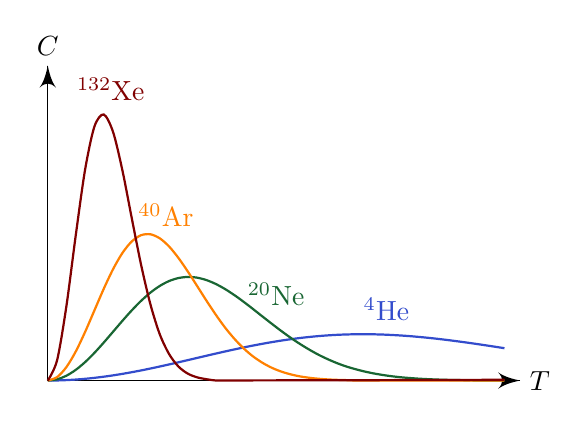
\begin{tikzpicture}
    \draw [->] (0, 0) -- (6, 0) node [right] {$T$};
    \draw [->] (0, 0) -- (0, 4) node [above] {$C$};

    \foreach \m/\colour in {4/mblue, 20/mgreen, 40/morange, 132/mred} {
      \draw [\colour, thick, domain=0:5.8, samples=50] plot [smooth] (\x, {1/10 * (\m/4)^(3/2) * \x^2 * exp (-\m / 4 * (\x^2 / 16))});
    }
    \node [mblue] at (4.3, 0.9) {$^{4}$He};
    \node [mgreen] at (2.9, 1.1) {$^{20}$Ne};
    \node [morange] at (1.5, 2.1) {$^{40}$Ar};
    \node [mred] at (0.8, 3.7) {$^{132}$Xe};
  \end{tikzpicture}
\end{center}
We see that the energy distribution shifts to the right as we increase the mass. This is expected, because we know that the energy of the particle is always $\frac{1}{2}kT$, and so for lighter particles, we need to have higher energy.

We can sanity-check that the expected value of $v$ is correct. We have
\[
  \bra v^2\ket = \int_0^\infty v^2 f(v) \;\d v = \frac{3kT}{m}.
\]
So we find that
\[
  \bra E\ket = \frac{1}{2} m\bra v^2\ket = \frac{3}{2} kT.
\]
This agrees with the equipartition of energy, as it must. But now we have an actual distribution, we can compute other quantities like $\bra v^4\ket$.

Note that in these derivations, we assumed we were dealing with a monoatomic ideal gas, but it happens that in fact this holds for a much more general family of gases. We will not go much into detail.

\subsection{Diatomic gases}
We now move on to consider more complicated gases. If we have molecules, then they can contain other forms of energy such as rotational energy.

Everything we are doing is classical, so we need to come up with a model of a diatomic molecule, instead of studying the actual quantum system of molecules. For simplicity, we can model them as two point masses joined together by a massless spring.
\begin{center}
  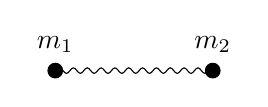
\begin{tikzpicture}
    \fill circle [radius=0.1];
    \fill (2, 0) circle [radius=0.1];
    \node [above] at (0, 0.1) {$m_1$};
    \node [above] at (2, 0.1) {$m_2$};
    \draw [decorate, decoration={snake, amplitude=1, segment length=5}] (0, 0) -- (2, 0);
  \end{tikzpicture}
\end{center}
As we know from classical dynamics, we can decompose the motion into different components:
\begin{itemize}
  \item Translation of the center of mass. We can view this as a single mass with energy $M = m_1 + m_2$.
  \item Rotations about center of mass. There are two axes of rotations orthogonal to the spring, and these have a moment of inertia $I$. We will ignore the rotation along the axes parallel to the spring because we assume the masses are point masses.
  \item Vibrations along the axis of symmetry. The important quantity here is the reduced mass
    \[
      m = \frac{m_1 m_1}{m_1 + m_2}.
    \]
\end{itemize}
We will assume all these motions are independent. In reality, the translation is indeed independent from the others, but the rotations and vibrations can couple in complicated ways. But with this assumption, we have
\[
  Z_1 = Z_{\mathrm{trans}} Z_{\mathrm{rot}} Z_{\mathrm{vib}}.
\]
We can obtain $Z_{\mathrm{trans}}$ just as the partition energy we obtained previously for a single mass, with mass $M$. The remaining two terms depend only on the relative position of the masses. So they do not depend on the molecule as a whole, and are going to be independent of $V$.

Now when we differentiate $\log Z_1$ with respect to $V$, then the latter two terms drop out, and thus we deduce that the ideal gas law still holds for diatomic gases.

We now try to figure out how rotations and vibrations contribute to the partition function. For rotations, we can parametrize this using spherical polars $(\theta, \varphi)$. The Lagrangian for this rotational motion is given by
\[
  \mathcal{L}_{\mathrm{rot}} = \frac{1}{2} I (\dot{\theta}^2 + \sin^2 \theta \dot{\varphi}^2).
\]
The conjugate momenta are given by
\begin{align*}
  p_\theta &= \frac{\partial \mathcal{L}}{\partial \dot{\theta}} = I \dot{\theta}\\
  p_\varphi &= \frac{\partial \mathcal{L}}{\partial \dot{\varphi}} = I \sin^2 \theta \dot\varphi.
\end{align*}
So we have
\[
  H_{\mathrm{rot}} = \dot{\theta} p_\theta + \dot{\varphi} p_\varphi - \mathcal{L}_{\mathrm{rot}} = \frac{p_\theta^2}{2I} + \frac{p_\varphi^2}{2I \sin^2 \theta}.
\]
We can then work out the partition function
\[
  Z_{\mathrm{rot}} = \frac{1}{(2\pi \hbar)^2} \int \d \theta\; \d \varphi\; \d p_\theta \; d p_\varphi\; e^{-\beta H_{\mathrm{rot}}}
\]
We note that the $p_\theta$ and $p_\varphi$ integrals are just Gaussians, and so we get
\[
  Z_{\mathrm{rot}} = \frac{1}{(2\pi \hbar)^2} \sqrt{\frac{2\pi I}{\beta}} \int_0^\pi \d \theta \sqrt{\frac{2\pi I \sin^2 \theta}{\beta}} \int_0^{2\pi} \d \varphi = \frac{2IkT}{\hbar^2}.
\]
Then we get
\[
  E_{\mathrm{rot}} = - \frac{\partial}{\partial \beta} \log Z_{\mathrm{rot}} = \frac{1}{\beta} = kT.
\]
This agrees with the equipartition of energy, as here we have two degrees of freedom, and each contributes $\frac{1}{2}kT$.

\begin{eg}
  In the case of a system where vibrations are not important, eg. if the string is very rigid, then we are done, and we have found
  \[
    Z = Z_{\mathrm{trans}} Z_{\mathrm{rot}} \propto (kT)^{5/2}.
  \]
  Then the partition function for $N$ particles is
  \[
    Z = \frac{1}{N!} Z_1^N.
  \]
  and the total energy is
  \[
    -\frac{\partial}{\partial \beta} \log Z = \frac{5}{2} NkT.
  \]
  This is exactly as we expect. There is $\frac{3}{2}NkT$ from translation, and $NkT$ from rotation. From this, we obtain the heat capacity
  \[
    C_V = \frac{5}{2} Nk.
  \]
\end{eg}
We now put in the vibrations. Since we are modelling it by a spring, we can treat it as a harmonic oscillator, with mass $m$ and frequency $\omega$, which is determined by the bond strength. Then if we let $\zeta$ be the displacement form equilibrium, then the Hamiltonian is
\[
  H_{\mathrm{vib}} = \frac{p_\zeta^2}{2m} + \frac{1}{2}m \omega^2 \zeta^2.
\]
So we have
\[
  Z_{\mathrm{fib}} = \frac{1}{2\pi \hbar} \int \d \zeta \d p_\zeta e^{-\beta H_{\mathrm{vib}}} = \frac{kT}{\hbar \omega}.
\]
From the partition function, we can get the energy of a single molecule, and find it to be
\[
  E_{\mathrm{vib}} = kT.
\]
This is the average energy in the vibrational motion of a molecule. This looks a bit funny. The vibration is only one degree of freedom, but the equipartition of energy seems to think this has two degrees of freedom. It turns out equipartition of energy behaves differently when we have potential energy. In general, we should think of having one degree of freedom for each quadratic term in the Hamiltonian, and so we have one degree of freedom for kinetic energy and another for potential.

Putting all three types of motion together, we get
\[
  E = \frac{7}{2} NkT,
\]
and the heat capacity is
\[
  C_V- = \frac{7}{2}Nk.
\]
Note that these results are completely independent of the parameters describing the molecule.

Does this agree with experiments? The answer is no! If we go and measure the heat capacity of, say, molecular hydrogen, we find something like
\begin{center}
  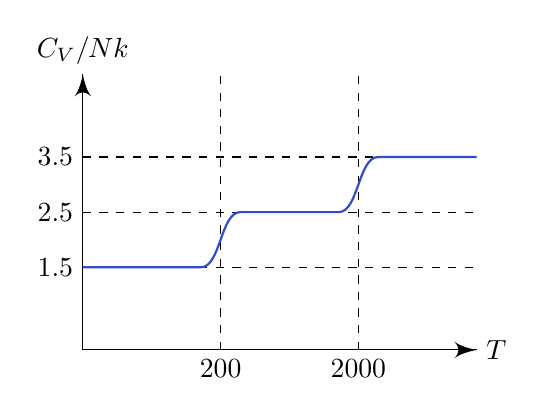
\begin{tikzpicture}[yscale=0.7]
    \draw [->] (0, 0) -- (5, 0) node [right] {$T$};
    \draw [->] (0, 0) -- (0, 5) node [above] {$C_V/Nk$};

    \draw [dashed] (1.75, 0) node [below] {$200$} -- +(0, 5);
    \draw [dashed] (3.5, 0) node [below] {$2000$} -- +(0, 5);

    \draw [dashed] (0, 1.5) node [left] {$1.5$} -- +(5, 0);
    \draw [dashed] (0, 2.5) node [left] {$2.5$} -- +(5, 0);
    \draw [dashed] (0, 3.5) node [left] {$3.5$} -- +(5, 0);

    \draw [thick, mblue] (0, 1.5) -- (1.5, 1.5) .. controls (1.75, 1.5) and (1.75, 2.5) .. (2, 2.5) -- (3.25, 2.5) .. controls (3.5, 2.5) and (3.5, 3.5) .. (3.75, 3.5) -- (5, 3.5);;
  \end{tikzpicture}
\end{center}
So it seems like our prediction only works when we have high enough temperature. At lower temperatures, the vibration modes freeze out. Then as we further lower the energy, rotation modes also go away. This is a big puzzle classically! This is explained by quantum effects, which we will discuss later.

\subsection{Interacting gases}
So far, we have been talking about ideal gases. What happens if there \emph{are} interactions?

For a real gas, if they are sufficiently dilute, ie. $N/V$ is small, then we expect the interactions to be negligible. This suggests that we can try to capture the effects of interactions perturbatively in $\frac{N}{V}$. We can write
\[
  \frac{p}{kT} = \frac{N}{V}.
\]
We can think of this as a first term in an expansion, and add higher order terms
\[
  \frac{p}{kT} = \frac{N}{V} + B_2(T) \frac{N^2}{V^2} + B_3 (T) \frac{N^3}{V^3} + \cdots.
\]
Note that the coefficients depend on $T$ only, as they should be intensive quantities. This is called the \term{Virial expansion}, and the coefficients $B_k(T)$ are the \term{Virial coefficients}. Our goal is to figure out what these $B_k(T)$ are.

We suppose the interaction is given by a potential energy $U(r)$ between two neutral atoms (assuming monoatomic) at separation $r$.

\begin{eg}
  In genuine atoms, for large $r$ (relative to atomic size), we have
  \[
    U(r) \propto -\frac{1}{r^6}.
  \]
  This comes from dipole-dipole interactions. Heuristically, we can understand this power of $6$ as follows --- while the expectation values of electric dipole of an atom vanishes, there exists non-trivial probability that the dipole $p_1$ is non-zero. This gives an electric field of
  \[
    E \sim \frac{p_1}{r^3}.
  \]
  This induces a dipole $p_2$ in atom $2$. So we have
  \[
    p_2 \propto E \sim \frac{p_1}{r^3}.
  \]
  So the resulting potential energy is
  \[
    U \propto -p_2 E \sim -\frac{p_1^2}{r^6}.
  \]
  This is called the \term{van der Waals interaction}. Note that the negative sign means this is an attractive force.

  For small $r$, the electron orbitals of the atoms start to overlap, and then we get repulsion due to the Pauli principle. All together, we obtain the \term{Lennard-Jones potential} given by
  \[
    U(r) = U_0\left(\left(\frac{r_0}{r}\right)^{12} - \left(\frac{r_0}{r}\right)^6\right).
  \]
  \begin{center}
    \begin{tikzpicture}
      \draw [->] (0, 0) -- (5, 0) node [right] {$r$};
      \draw [->] (0, -2) -- (0, 2) node [above] {$U(r)$};

      \draw [mblue, thick ] plot coordinates {(0.955,2.00000) (0.960,1.77280) (0.965,1.47565) (0.970,1.20365) (0.975,0.95482) (0.980,0.72738) (0.985,0.51965) (0.990,0.33010) (0.995,0.15732) (1.000,0.00000) (1.005,-0.14306) (1.010,-0.27298) (1.015,-0.39077) (1.020,-0.49739) (1.025,-0.59370) (1.030,-0.68052) (1.035,-0.75859) (1.040,-0.82859) (1.045,-0.89116) (1.050,-0.94689) (1.055,-0.99632) (1.060,-1.03996) (1.065,-1.07826) (1.070,-1.11165) (1.075,-1.14054) (1.080,-1.16528) (1.085,-1.18622) (1.090,-1.20366) (1.095,-1.21791) (1.100,-1.22922) (1.105,-1.23784) (1.110,-1.24400) (1.115,-1.24792) (1.120,-1.24978) (1.125,-1.24977) (1.130,-1.24806) (1.135,-1.24480) (1.140,-1.24014) (1.145,-1.23420) (1.150,-1.22710) (1.155,-1.21897) (1.160,-1.20990) (1.165,-1.19999) (1.170,-1.18932) (1.175,-1.17799) (1.180,-1.16606) (1.185,-1.15361) (1.190,-1.14069) (1.195,-1.12737) (1.200,-1.11371) (1.205,-1.09974) (1.210,-1.08553) (1.215,-1.07110) (1.220,-1.05650) (1.225,-1.04177) (1.230,-1.02693) (1.235,-1.01202) (1.240,-0.99707) (1.245,-0.98210) (1.250,-0.96712) (1.255,-0.95217) (1.260,-0.93727) (1.265,-0.92242) (1.270,-0.90764) (1.275,-0.89296) (1.280,-0.87837) (1.285,-0.86390) (1.290,-0.84956) (1.295,-0.83534) (1.300,-0.82127) (1.305,-0.80735) (1.310,-0.79358) (1.315,-0.77997) (1.320,-0.76652) (1.325,-0.75325) (1.330,-0.74015) (1.335,-0.72722) (1.340,-0.71448) (1.345,-0.70191) (1.350,-0.68953) (1.355,-0.67733) (1.360,-0.66532) (1.365,-0.65349) (1.370,-0.64184) (1.375,-0.63039) (1.380,-0.61911) (1.385,-0.60803) (1.390,-0.59712) (1.395,-0.58640) (1.400,-0.57586) (1.405,-0.56550) (1.410,-0.55532) (1.415,-0.54531) (1.420,-0.53548) (1.425,-0.52583) (1.430,-0.51635) (1.435,-0.50703) (1.440,-0.49789) (1.445,-0.48891) (1.450,-0.48009) (1.455,-0.47144) (1.460,-0.46294) (1.465,-0.45460) (1.470,-0.44642) (1.475,-0.43838) (1.480,-0.43050) (1.485,-0.42277) (1.490,-0.41518) (1.495,-0.40773) (1.500,-0.40042) (1.530,-0.35940) (1.560,-0.32284) (1.590,-0.29030) (1.620,-0.26131) (1.650,-0.23550) (1.680,-0.21250) (1.710,-0.19198) (1.740,-0.17367) (1.770,-0.15732) (1.800,-0.14268) (1.830,-0.12958) (1.860,-0.11784) (1.890,-0.10729) (1.920,-0.09782) (1.950,-0.08929) (1.980,-0.08160) (2.010,-0.07467) (2.040,-0.06841) (2.070,-0.06275) (2.100,-0.05762) (2.130,-0.05297) (2.160,-0.04875) (2.190,-0.04491) (2.220,-0.04142) (2.250,-0.03824) (2.280,-0.03534) (2.310,-0.03269) (2.340,-0.03027) (2.370,-0.02806) (2.400,-0.02603) (2.430,-0.02417) (2.460,-0.02246) (2.490,-0.02089) (2.520,-0.01945) (2.550,-0.01812) (2.580,-0.01690) (2.610,-0.01577) (2.640,-0.01473) (2.670,-0.01376) (2.700,-0.01287) (2.730,-0.01205) (2.760,-0.01129) (2.790,-0.01058) (2.820,-0.00992) (2.850,-0.00931) (2.880,-0.00875) (2.910,-0.00822) (2.940,-0.00773) (2.970,-0.00727) (3.000,-0.00685) (3.100,-0.00563) (3.200,-0.00465) (3.300,-0.00387) (3.400,-0.00323) (3.500,-0.00272) (3.600,-0.00230) (3.700,-0.00195) (3.800,-0.00166) (3.900,-0.00142) (4.000,-0.00122) (4.100,-0.00105) (4.200,-0.00091) (4.300,-0.00079) (4.400,-0.00069) (4.500,-0.00060) (4.600,-0.00053) (4.700,-0.00046) (4.800,-0.00041) (4.900,-0.00036) (5.000,-0.00032)};

    % map (\x -> (showFFloat (Just 3) x "", showFFloat (Just 5) (min 2 (5 * (1/(x^12) - 1/(x^6)))) "")) [0.955,0.96..1.5]
    % map (\x -> (showFFloat (Just 3) x "", showFFloat (Just 5) (5 * (1/(x^12) - 1/(x^6))) "")) [1.53,1.56..3]
    % map (\x -> (showFFloat (Just 3) x "", showFFloat (Just 5) (5 * (1/(x^12) - 1/(x^6))) "")) [3.1,3.2..5]
    \end{tikzpicture}
  \end{center}
  To make life easy, we will actually use a ``hard core repulsion'' potential instead, given by
  \[
    U(r) =
    \begin{cases}
      \infty & r < r_0\\
      -U_0 \left(\frac{r_0}{r}\right)^6 & r > r_0
    \end{cases}
  \]
  \begin{center}
    \begin{tikzpicture}
      \draw [->] (0, 0) -- (5, 0) node [right] {$r$};
      \draw [->] (0, -2) -- (0, 2) node [above] {$U(r)$};

      \draw [mblue, thick, domain=0.9:5, samples=50] plot [smooth] (\x, {-1/\x^6});

      \draw [mblue, thick] (0.9, -1.8817) -- (0.9, 2);

      \node [anchor = north east] at (0.9, 0) {$r_0$};
    \end{tikzpicture}
  \end{center}
\end{eg}
For a general $U$, we can write the Hamiltonian of the gas is
\[
  H = \sum_{i = 1}^N \frac{\mathbf{p}_i^2}{2m} + \sum_{i > j} U(r_{ij}),
\]
with
\[
  r_{ij} = |\mathbf{r}_i - \mathbf{r}_j|.
\]
is the separation between particle $i$ and particle $j$.

Because of this interaction, it is no longer the case that the partition function for $N$ particles is the $N$th power of the partition function for one particle. We have
\begin{align*}
  Z(N, V, T) &= \frac{1}{N} \frac{1}{(2\pi \hbar)^{3n}} \int \prod_{i = 1}^N \d^3 p_i\; \d^3 r_i e^{-\beta H}\\
  &= \frac{1}{N!} \frac{1}{(2\pi \hbar)^{3n}} \left(\int \prod_{i} \d^3 p_i e^{-\beta p_i^2/2m}\right)\left(\int \prod_i \d^3 r_i\; e^{-\beta \sum_{j < k} U(r_{ij})} \right)\\
  &= \frac{1}{N! \lambda^{3N}} \int \prod_i \d^3 r_i\; e^{-\beta \sum_{j < k} U(r_{ij})},
\end{align*}
where again
\[
  \lambda = \sqrt{\frac{2\pi \hbar^2}{mkT}}.
\]
Since we want to get an expansion, we might want to expand this in terms of the potential, but that is not helpful, because the potential is infinite for small $r$. Instead it is useful to consider the \term{Mayer $f$-function}:
\[
  f(r) = e^{-\beta U(r)} - 1.
\]
This function has the property that $f(r) = -1$ for $r < r_0$ (in the case of the hardcore repulsion), and $f(r) \to 0$ as $r \to \infty$. So this is a nicer function as it only varies within this finite range.

We further simplify notatino by defining
\[
  f_{ij} = f(r_{ij}).
\]
Then we have
\begin{align*}
  Z(N, V, T) &= \frac{1}{N! \lambda^{3N}} \left(\prod_i \d^3 r_i\prod_{j < k} (1 + f_{jk})\right)\\
  &= \frac{1}{N!\lambda^{3N}} \int \prod_i \d^3 r_i \left(1 + \sum_{j < k} f_{jk} + \sum_{j < k} \sum_{\ell < m} f_{jk} f_{\ell m} + \cdots\right).
\end{align*}
The first term is just
\[
  \int \prod_i \d^3 r_i = V^N,
\]
and this gives the ideal gas term. Now each of the second terms is the same, eg. for $j = 1, k = 2$, this is
\[
  \int \prod_i \d^3 r_i f_{12} = V^{N - 2} \int \d^3 r_1 \; \d^3 r_2\; f_{12} = V^{N - 1} I,
\]
where we set
\[
  I = \int\d^3 r f(r).
\]
Since $f(r) \to 0$ as $r \to \infty$, we might as well integrate over all space. Summing over all terms, and approximating $N(N - 1)/2 \sim N^2/2$, we find that the first two terms of the partition function are
\[
  Z(N, V, T) = \frac{V^N}{N! \lambda^{3N}} \left(1 + \frac{N^2}{2V}I + \cdots\right).
\]
Up to first order, we can write this as
\begin{align*}
  Z(N, V, T) &= \frac{V^N}{N! \lambda^{3N}} \left(1 + \frac{N}{2V}I + \cdots\right)^N\\
  &= Z_{\mathrm{ideal}} \left(1 + \frac{N}{2V}I + \cdots \right)^N.
\end{align*}
This pulling out of the $N$ to the exponent might seem a bit arbitrary, but writing it this way, it makes it much clearer that $S$, $F$ etc would be extensive quantities. For example, we can write down the free energy as
\[
  F = -kT \log Z = F_{\mathrm{ideal}} - NkT \log \left(1 + \frac{N}{2V} I + \cdots\right).
\]
Without actually computing $I$, we can expect that it grows as $I \sim r_0^3$. Since we are expanding in terms of $NI/V$, we need
\[
  \frac{N}{V} \ll \frac{1}{r_0^3}.
\]
So we know the expansion is valid if the density of the gas is much less than the density of an atom. In real life, to determine the density of an atom, we need to find a system where the atoms are closely packed. Thus, it suffices to measure the density of the substance in liquid or solid form.

Assuming that the gas is indeed not dense, we can further use the approximation
\[
  \log(1 + x) \approx x.
\]
So we have
\[
  p = - \left(\frac{\partial F}{\partial V}\right)_T = \frac{NkT}{V}\left(1 - \frac{N}{2V} I + \cdots\right).
\]
So we have
\[
  \frac{pV}{NkT} = 1 - \frac{N}{2V} I + \cdots.
\]
So we can now read off what the second Virial coefficient is:
\[
  B_2 = -\frac{1}{2} I.
\]
We can consdier what we get with different potential. If we have a completely repulsive potential, then $U(r) > 0$ everywhere. So $f < 0$, and thus $B_2(t) > 0$. In other words, having a repulsive interaction tends to increase the pressure, which makes sense. On the other hand, if we have an attractive potential, then the pressure decreases.

If we have a hardcore repulsion, then we have
\[
  I = \int_{r = 0}^{r = r_0} \d^3 r\; (-1) + \int_{r = r_0}^\infty \d^3 r\; \left(e^{\beta U_0 (r_0/r)^6} - 1\right).
\]
The second term is slightly tricky, so we'll restrict to the case of high temperature, hence small $\beta$. We can write
\[
  e^{\beta U_0 (r_0/r)^6} \approx 1 + \beta U_0 \left(\frac{r_0}{r}\right)^6 + \cdots
\]
Then we get
\[
  I \approx \frac{4}{3}\pi r_0^3 +\frac{4 \pi U_0}{kT} \int_{r_0}^\infty \d r\; \frac{r_0^6}{r^6} = \frac{4\pi r_0^3}{3}\left(\frac{U_0}{kT} - 1\right).
\]
For large $T$, this is negative, and so the repulsive interaction dominates. We can plug this into our equation of state, and find
\[
  \frac{pV}{NkT} \approx 1 - \frac{N}{V}\left(\frac{a}{kT} - b\right),
\]
where
\[
  a = \frac{2\pi r_0^3}{3}U_0,\quad b = \frac{2\pi r_0^3}{3}.
\]
We can invert this to get
\[
  kT = \frac{V}{N}\left(p + \frac{N^2}{V^2} a\right) \left(1 + \frac{N}{V}b\right)^{-1}.
\]
Taking the Taylor expansion of the inverse and truncating higher order terms, we obtain
\[
  kT = \left(p + \frac{N^2}{V^2}a \right)\left(\frac{V}{N} - b\right).
\]
This is the \term{van der Waals equation of state}\index{equation of state!van der waals}, which is valid at low density ($Nr_0^3/V \ll 1$) and high temperature ($\beta U_0 \ll 1$).

We can also write this as
\[
  p = \frac{NkT}{V - bN} - a \frac{N^2}{V^2}.
\]
and we see that $a$ gives a reduced pressure due to long distance attractive force, while we can view the $b$ contribution as saying that the atoms take up space, and hence reduces the volume.

By why exactly the factor of $bN$? Imagine two atoms living right next to each other.
\begin{center}
  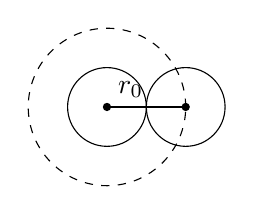
\begin{tikzpicture}[scale=0.5]
    \draw circle [radius=1];
    \draw (2, 0) circle [radius=1];
    \draw [dashed] circle [radius=2];

    \draw (0, 0) node [circ] {} -- (2, 0) node [circ] {} node [pos=0.3, above] {$r_0$};
  \end{tikzpicture}
\end{center}
The value $r_0$ was chosen to be the distance between the two cores, so the volume of each atom is
\[
  \frac{4\pi}{3}\left(\frac{r_0}{2}\right)^3,
\]
which is not $b$. We might think the right way to do this problem is to look at how much volume the atom excludes, ie. the dashed volume. This is
\[
  \Omega = \frac{4}{3}\pi r_0^3 = 2b.
\]
This is again not right. So we probably want to think more carefully.

Suppose we hae $N$ particles. When we put in the first atom, the amount of space available to put it is $V$. When we now tryr to put in the second, the available space is $V - \Omega$ (assuming the two atoms are not too close together so that they don't exclude the same volume). Similarly, when we put in the third, the available space is $V - 2 \Omega$.

Diving by $N!$ for indistinguishability, we find that the total phase space volume available for placing our particles is
\begin{align*}
  \frac{1}{N!}V(V - \Omega) (V -2\Omega) \cdots (V - (N - 1) \Omega) &\approx \frac{1}{N!} V^N\left(1 - \frac{N^2}{2} \frac{\Omega}{V} + \cdots\right)\\
  &\approx \frac{1}{N!} \left(V - \frac{N\Omega}{2}\right)^N,
\end{align*}
which explains why the reduced volume for each particle is $\Omega/2$ instead of $\Omega$.

The pure mathematics student who accidentally walked into this lecture hall would certainly complain that a lot of the stpes done in the derivation were not very rigorous. In particular, we just asserted that that the first-order terms in the expansion of $\prod (1 + f_{jk})$ was the terms $\sum f_{jk}$. While you might think this is obviously true, it happens that the second-order terms are \emph{not} the $\sum \sum f_{jk} f_{\ell m}$ terms. Thus we really want to keep track of the terms in the expansion carefully.

The way to do it properly would be via the \term{cluster expansion}, which involves using nice diagrams to figure out the right terms to include, similar to how Feynamn diagrams are used to do perturbation theory in quantum field theory. Unfortunately, we do not have the time to go into the details.


\section{Quantum gases}
We now move on to study quantum gases. We begin by discussing a slightly technical point.

\subsection{Density of states}
While the energy levels we talk about are technically discrete, they are in practice very close together, and it is more convenient to pretend they are continuous. When we do so, we have to be careful to preserve the ``density'' of the energy levels.

Consider an ideal gas in a cubic box with side lengths $L$. So we have $V = L^3$. Since there are no interactions, the wavefunction for multiple states can be obtained from the wavefunction of single particle states,
\[
  \psi(\mathbf{x}) = \frac{1}{\sqrt{V}} e^{i\mathbf{k}\cdot \mathbf{x}}.
\]
We impose periodic boundary conditions, so the wavevectors are quantized by
\[
  k_i = \frac{2\pi n_i}{L},
\]
with $n_i \in \Z$.

The one-particle energy is given by
\[
  E_\mathbf{n} = \frac{\hbar^2 \mathbf{k}^2}{2m} = \frac{4\pi^2 \hbar^2}{2mL^2}(n_1^2 + n_2^2 + n_3^2).
\]
So if we are interested in a one-particle partition function, we have
\[
  Z_1 = \sum_\mathbf{n} e^{-\beta E_\mathbf{n}}.
\]
We now note that
\[
  \beta E_n \sim \frac{\lambda^2}{L^2}\mathbf{n}^2,
\]
where
\[
  \lambda = \sqrt{\frac{2\pi \hbar^2}{mkT}}.
\]
is the de Broglie wavelength.

This $\frac{\lambda^2}{L^2}$ gives the spacing between the energy levels. But we know that $\lambda \ll L$. So the energy levels are very finely spaced, and we can replace the sum by an integral. Thus we can write
\[
  \sum_\mathbf{n} \approx \int \d^3 \mathbf{n} \approx \frac{V}{(2\pi)^3} \int \d^3 \mathbf{k} \approx \frac{4\pi V}{(2\pi)^3} \int_0^\infty \d |\mathbf{k}|\; |\mathbf{k}|^2,
\]
where in the last step, we replace with spherical polars and integrated over angles. The final step is to replace $|\mathbf{k}|$ by $E$. We know that
\[
  E = \frac{\hbar^2 |\mathbf{k}|^2}{2m}.
\]
So we get that
\[
  \d E = \frac{\hbar^2 |\mathbf{k}|}{m} \d |\mathbf{k}|.
\]
Therefore we can write
\[
  \sum_\mathbf{n} = \frac{4\pi V}{(2\pi)^3} \int_0^\infty \d E\; \sqrt{\frac{2mE}{\hbar^2}}\frac{m}{\hbar^2}.
\]
We then set
\[
  g(E) = \frac{V}{2\pi^2} \left(\frac{2m}{\hbar^2}\right)^{3/2} E^{1/2}.
\]
This is called the \term{density of states}. Approximately, $g(E) \;\d E$ is the number of single particle states with energy between $E$ and $E + \d E$.

All these derivations work if we have a non-relativistic free particle, since we assumed the \term{dispersion relation} between $E$ and $\mathbf{k}$, namely
\[
  E = \frac{\hbar^2 |\mathbf{k}|^2}{2m}.
\]
For a relativistic particle, we instead have
\[
  E = \sqrt{\hbar^2 |\mathbf{k}|^2 c^2 + m^2c^4}.
\]
In this case, $|\mathbf{k}|$ is still quantized as before, and repeating the previous argument, we find that
\[
  g(E) = \frac{VE}{2\pi^3 \hbar^3 c^3} \sqrt{E^2 - m^2 c^4}.
\]
We will be interested in the special case where $m = 0$. Then we simply have
\[
  g(E) = \frac{VE^2}{2\pi^3 \hbar^3 c^3}.
\]
We can start doing some physics with this.

\subsection{Black-body radiation}
We now suppose we have a gas of photons (which is just a fancy way to say ``photons'') in a box with opaque walls.
\begin{center}
  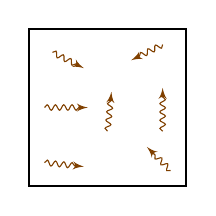
\begin{tikzpicture}[photon/.style={morange!50!black, decorate, decoration={snake, amplitude=1, segment length=3, post=lineto, post length=3}, -latex'}]
    \draw [thick] (0, 0) rectangle (2, 2);

    \draw [photon] (0.3, 1.7) -- +(0.4, -0.2);
    \draw [photon] (1, 0.7) -- +(0.05, 0.5);

    \draw [photon] (0.2, 0.3) -- +(0.5, -0.05);
    \draw [photon] (1.7, 0.7) -- +(0, 0.55);
    \draw [photon] (1.8, 0.2) -- +(-0.3, 0.3);
    \draw [photon] (0.2, 1) -- +(0.55, 0);
    \draw [photon] (1.7, 1.8) -- +(-0.4, -0.2);
  \end{tikzpicture}
\end{center}
We suppose this box of photon is at equilibrium with temperature $T$. We will use the box of photons as a model of a ``\term{black body}'', ie. a perfectly absorbing object. The gas of photons inside is called \term{black-body radiation}.
 Later on, we will argue that the photons emitted by a black body must indeed follow the same distribution as the photons inside our box.

We begin by reminding ourselves of some basic properties of photons: they are massless and have energy
\[
  E = \hbar \omega,\quad \omega = \frac{2\pi c}{\lambda},
\]
and $\lambda$ is the (genuine) wavelength of the photon.

Interactions between photons are negligible, so we can treat them as noble gas.

Photons have two polarization states, since given any direction of travel $\mathbf{k}$, the electric and magnetic fields have to obey
\[
  \mathbf{E} \cdot \mathbf{k} = \mathbf{B} \cdot \mathbf{k} = \mathbf{B} \cdot \mathbf{E} = 0,
\]
and there are two independent choices for $\mathbf{E}$ and $\mathbf{B}$. This has implications for our counting, as we need an extra factor of $2$ in our density of states. So the density of states is given by
\[
  g(E) \;\d E = \frac{VE^2}{\pi^2 \hbar^3 c^3}\;\d E.
\]
Using the fact that
\[
  E = \hbar \omega,
\]
it is often convenient to instead write this as
\[
  g(\omega)\; \d \omega = \frac{V \omega^2}{\pi^2 c^3}\;\d \omega.
\]
This is an abuse of notation, as the two $g$'s we wrote down are different functions, but this is a physics course.

The final important property of the photons is that photon numbers are not conserved. Indeed, they are absorbed and emitted by walls of the box. So we must sum over all possible photon numbers, even though we are in the canonical ensemble. In practice, what we get is the same as the grand canonical ensemble, but with $\mu = 0$.

We can begin. Let's forget about photons for the moment, and consider this problem more generally. Consider a system of non-interacting particles with one-particle states $\bket{i}$ of energies $E_i$. Then the general accessible state can be labelled by
\[
  \{n_1, n_2, \cdots\},
\]
where $n_i$ is the number of particles in $\bket{i}$. Since particle numbers are not conserved, we do not impose any restrictions on the possible values of the $n_i$. The energy of such a state is just
\[
  \sum_i n_i E_i.
\]
As before, in the canonical ensemble, the probability of being in such a state is
\[
  p(\{n_i\}) = \frac{1}{Z} e^{-\beta \sum n_j E_j},
\]
and
\[
  Z = \sum_{\{n_k\}} e^{-\beta \sum n_j E_j} = \sum_{n_1 = 0}^\infty e^{-\beta n_1 E_1} \sum_{n = 2}^\infty e^{-\beta n_2 E_2} \cdots = \prod_i \frac{1}{1 - e^{-\beta E_i}}.
\]
So we find that
\[
  \log Z = - \sum_i \log (1 - e^{-\beta E_i}).
\]
Using this, we have
\begin{align*}
  \bra n_i\ket &= \sum_{\{n_k\}} n_i p (\{n_k\}) \\
  &= \sum_{\{n_k\}} \frac{n_i e^{-\beta \sum_j n_j E_j}}{Z}\\
  &= - \frac{1}{\beta} \frac{\partial}{\partial E_i} \log Z.
\end{align*}
Using the formula of $\log Z$ we had, we find
\[
  \bra n_i\ket = \frac{1}{e^{\beta E_i} - 1}.
\]
Applying this to photons, we replace the sum with an integral, and $E_i = \hbar \omega$. Using our density of states, we have
\[
  \log Z = - \frac{V}{\pi^3 c^3} \int_0^\infty \d \omega\; \omega^2 \log(1 - e^{-\beta \hbar \omega}).
\]
Similarly, the average number of photons with frequency between $\omega$ and $\d \omega$ is
\[
  n(\omega)\; \d \omega = g(\omega) \;\d \omega \cdot \frac{1}{e^{\beta \hbar \omega} - 1} = \frac{V \omega^2\;\d \omega}{\pi^2 c^3(e^{\beta\hbar\omega} - 1)}.
\]
Thus, the total energy in this range is
\[
  E(\omega) \;\d \omega = \hbar \omega n(\omega) \;\d \omega = \frac{V \hbar}{\pi^2 c^3} \frac{\omega^3}{e^{\beta \hbar \omega} - 1}\;\d \omega.
\]
This is the \term{Planck distribution}.

Let's check that this makes sense. Let's try to compute the total energy of all photons. We have
\[
  E = -\left(\frac{\partial \log Z}{\partial \beta}\right)_V = \frac{V \hbar}{\pi^2 c^3}\int_0^\infty \d \omega\; \frac{\omega^3}{e^{\beta \hbar \omega} - 1} = \int_0^\infty E(\omega) \;\d \omega,
\]
as we would expect.

Putting $\omega = \frac{2\pi c}{\lambda}$, we find that the average energy with wavelength between $\lambda$ and $\lambda + \d \lambda$ is given by the horrendous formula
\[
  \tilde{E} (\lambda) \;\d \lambda = \frac{V \hbar (2\pi c)^4}{\pi^2 c^3 \lambda^5} \frac{\d \lambda}{e^{\beta \hbar 2 \pi c/\lambda} - 1}.
\]
We can plot this for some values of $T$:
\begin{center}
  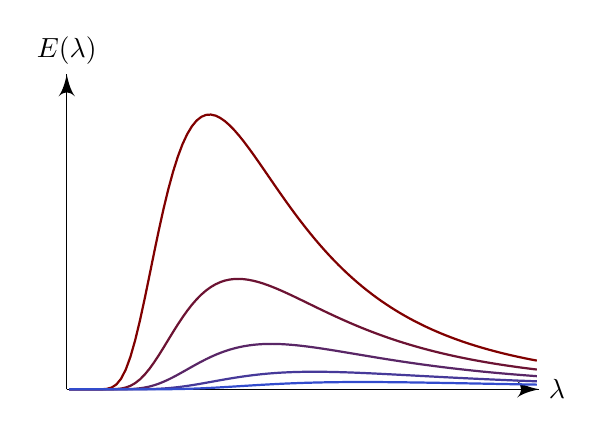
\begin{tikzpicture}[xscale=3]
    \draw [->] (0, 0) -- (2, 0) node [right] {$\lambda$};

    \draw [->] (0, 0) -- (0, 4) node [above] {$E(\lambda)$};

    \draw [mred, thick] plot coordinates {(0.01,0.00000) (0.03,0.00000) (0.05,0.00000) (0.07,0.00000) (0.09,0.00000) (0.11,0.00000) (0.13,0.00010) (0.15,0.00109) (0.17,0.00611) (0.19,0.02244) (0.21,0.06120) (0.23,0.13450) (0.25,0.25167) (0.27,0.41663) (0.29,0.62717) (0.31,0.87585) (0.33,1.15188) (0.35,1.44304) (0.37,1.73730) (0.39,2.02399) (0.41,2.29438) (0.43,2.54192) (0.45,2.76219) (0.47,2.95266) (0.49,3.11234) (0.51,3.24152) (0.53,3.34137) (0.55,3.41373) (0.57,3.46083) (0.59,3.48514) (0.61,3.48919) (0.63,3.47550) (0.65,3.44649) (0.67,3.40444) (0.69,3.35144) (0.71,3.28941) (0.73,3.22004) (0.75,3.14488) (0.77,3.06525) (0.79,2.98233) (0.81,2.89713) (0.83,2.81052) (0.85,2.72324) (0.87,2.63592) (0.89,2.54907) (0.91,2.46314) (0.93,2.37848) (0.95,2.29538) (0.97,2.21406) (0.99,2.13472) (1.01,2.05748) (1.03,1.98244) (1.05,1.90968) (1.07,1.83922) (1.09,1.77111) (1.11,1.70532) (1.13,1.64185) (1.15,1.58068) (1.17,1.52177) (1.19,1.46506) (1.21,1.41052) (1.23,1.35808) (1.25,1.30769) (1.27,1.25928) (1.29,1.21279) (1.31,1.16816) (1.33,1.12531) (1.35,1.08419) (1.37,1.04473) (1.39,1.00687) (1.41,0.97054) (1.43,0.93569) (1.45,0.90225) (1.47,0.87016) (1.49,0.83938) (1.51,0.80984) (1.53,0.78149) (1.55,0.75429) (1.57,0.72818) (1.59,0.70312) (1.61,0.67906) (1.63,0.65596) (1.65,0.63378) (1.67,0.61247) (1.69,0.59201) (1.71,0.57235) (1.73,0.55346) (1.75,0.53530) (1.77,0.51785) (1.79,0.50108) (1.81,0.48494) (1.83,0.46943) (1.85,0.45450) (1.87,0.44014) (1.89,0.42633) (1.91,0.41303) (1.93,0.40022) (1.95,0.38789) (1.97,0.37602) (1.99,0.36458)};
    \draw [mred!75!mblue, thick] plot coordinates {(0.01,0.00000) (0.03,0.00000) (0.05,0.00000) (0.07,0.00000) (0.09,0.00000) (0.11,0.00000) (0.13,0.00000) (0.15,0.00002) (0.17,0.00018) (0.19,0.00095) (0.21,0.00351) (0.23,0.00990) (0.25,0.02283) (0.27,0.04515) (0.29,0.07922) (0.31,0.12643) (0.33,0.18696) (0.35,0.25984) (0.37,0.34317) (0.39,0.43442) (0.41,0.53075) (0.43,0.62931) (0.45,0.72742) (0.47,0.82274) (0.49,0.91332) (0.51,0.99764) (0.53,1.07459) (0.55,1.14345) (0.57,1.20381) (0.59,1.25557) (0.61,1.29883) (0.63,1.33386) (0.65,1.36107) (0.67,1.38097) (0.69,1.39409) (0.71,1.40103) (0.73,1.40238) (0.75,1.39871) (0.77,1.39061) (0.79,1.37861) (0.81,1.36323) (0.83,1.34492) (0.85,1.32414) (0.87,1.30127) (0.89,1.27669) (0.91,1.25071) (0.93,1.22363) (0.95,1.19571) (0.97,1.16717) (0.99,1.13822) (1.01,1.10904) (1.03,1.07978) (1.05,1.05056) (1.07,1.02152) (1.09,0.99274) (1.11,0.96431) (1.13,0.93629) (1.15,0.90875) (1.17,0.88173) (1.19,0.85528) (1.21,0.82941) (1.23,0.80415) (1.25,0.77953) (1.27,0.75555) (1.29,0.73221) (1.31,0.70953) (1.33,0.68750) (1.35,0.66611) (1.37,0.64537) (1.39,0.62527) (1.41,0.60578) (1.43,0.58692) (1.45,0.56865) (1.47,0.55097) (1.49,0.53387) (1.51,0.51733) (1.53,0.50133) (1.55,0.48587) (1.57,0.47092) (1.59,0.45648) (1.61,0.44252) (1.63,0.42903) (1.65,0.41599) (1.67,0.40340) (1.69,0.39123) (1.71,0.37948) (1.73,0.36812) (1.75,0.35716) (1.77,0.34656) (1.79,0.33632) (1.81,0.32643) (1.83,0.31687) (1.85,0.30763) (1.87,0.29871) (1.89,0.29008) (1.91,0.28175) (1.93,0.27369) (1.95,0.26590) (1.97,0.25837) (1.99,0.25109)};
    \draw [mred!50!mblue, thick] plot coordinates {(0.01,0.00000) (0.03,0.00000) (0.05,0.00000) (0.07,0.00000) (0.09,0.00000) (0.11,0.00000) (0.13,0.00000) (0.15,0.00000) (0.17,0.00000) (0.19,0.00002) (0.21,0.00013) (0.23,0.00047) (0.25,0.00139) (0.27,0.00338) (0.29,0.00709) (0.31,0.01322) (0.33,0.02241) (0.35,0.03516) (0.37,0.05174) (0.39,0.07217) (0.41,0.09624) (0.43,0.12354) (0.45,0.15350) (0.47,0.18547) (0.49,0.21877) (0.51,0.25270) (0.53,0.28661) (0.55,0.31991) (0.57,0.35209) (0.59,0.38274) (0.61,0.41150) (0.63,0.43812) (0.65,0.46243) (0.67,0.48432) (0.69,0.50373) (0.71,0.52066) (0.73,0.53515) (0.75,0.54728) (0.77,0.55713) (0.79,0.56484) (0.81,0.57053) (0.83,0.57433) (0.85,0.57639) (0.87,0.57685) (0.89,0.57585) (0.91,0.57354) (0.93,0.57003) (0.95,0.56547) (0.97,0.55997) (0.99,0.55365) (1.01,0.54660) (1.03,0.53893) (1.05,0.53072) (1.07,0.52206) (1.09,0.51303) (1.11,0.50369) (1.13,0.49410) (1.15,0.48433) (1.17,0.47441) (1.19,0.46440) (1.21,0.45434) (1.23,0.44426) (1.25,0.43420) (1.27,0.42418) (1.29,0.41423) (1.31,0.40436) (1.33,0.39461) (1.35,0.38497) (1.37,0.37548) (1.39,0.36613) (1.41,0.35694) (1.43,0.34792) (1.45,0.33907) (1.47,0.33040) (1.49,0.32191) (1.51,0.31360) (1.53,0.30549) (1.55,0.29755) (1.57,0.28981) (1.59,0.28226) (1.61,0.27489) (1.63,0.26770) (1.65,0.26071) (1.67,0.25389) (1.69,0.24725) (1.71,0.24078) (1.73,0.23449) (1.75,0.22837) (1.77,0.22242) (1.79,0.21663) (1.81,0.21100) (1.83,0.20553) (1.85,0.20021) (1.87,0.19504) (1.89,0.19001) (1.91,0.18513) (1.93,0.18038) (1.95,0.17577) (1.97,0.17129) (1.99,0.16693)};

    \draw [mred!25!mblue, thick] plot coordinates {(0.01,0.00000) (0.03,0.00000) (0.05,0.00000) (0.07,0.00000) (0.09,0.00000) (0.11,0.00000) (0.13,0.00000) (0.15,0.00000) (0.17,0.00000) (0.19,0.00000) (0.21,0.00000) (0.23,0.00001) (0.25,0.00004) (0.27,0.00012) (0.29,0.00032) (0.31,0.00072) (0.33,0.00147) (0.35,0.00269) (0.37,0.00454) (0.39,0.00718) (0.41,0.01072) (0.43,0.01523) (0.45,0.02077) (0.47,0.02733) (0.49,0.03485) (0.51,0.04326) (0.53,0.05244) (0.55,0.06226) (0.57,0.07257) (0.59,0.08321) (0.61,0.09404) (0.63,0.10491) (0.65,0.11569) (0.67,0.12625) (0.69,0.13649) (0.71,0.14632) (0.73,0.15567) (0.75,0.16446) (0.77,0.17267) (0.79,0.18025) (0.81,0.18719) (0.83,0.19347) (0.85,0.19910) (0.87,0.20407) (0.89,0.20841) (0.91,0.21213) (0.93,0.21526) (0.95,0.21781) (0.97,0.21982) (0.99,0.22132) (1.01,0.22234) (1.03,0.22290) (1.05,0.22305) (1.07,0.22281) (1.09,0.22221) (1.11,0.22128) (1.13,0.22005) (1.15,0.21855) (1.17,0.21680) (1.19,0.21483) (1.21,0.21266) (1.23,0.21032) (1.25,0.20781) (1.27,0.20518) (1.29,0.20242) (1.31,0.19956) (1.33,0.19661) (1.35,0.19359) (1.37,0.19051) (1.39,0.18738) (1.41,0.18421) (1.43,0.18102) (1.45,0.17781) (1.47,0.17459) (1.49,0.17137) (1.51,0.16815) (1.53,0.16494) (1.55,0.16175) (1.57,0.15858) (1.59,0.15544) (1.61,0.15233) (1.63,0.14924) (1.65,0.14620) (1.67,0.14319) (1.69,0.14023) (1.71,0.13730) (1.73,0.13443) (1.75,0.13159) (1.77,0.12881) (1.79,0.12607) (1.81,0.12338) (1.83,0.12074) (1.85,0.11815) (1.87,0.11561) (1.89,0.11311) (1.91,0.11067) (1.93,0.10828) (1.95,0.10594) (1.97,0.10364) (1.99,0.10140)};

    \draw [mblue, thick] plot coordinates {(0.01,0.00000) (0.03,0.00000) (0.05,0.00000) (0.07,0.00000) (0.09,0.00000) (0.11,0.00000) (0.13,0.00000) (0.15,0.00000) (0.17,0.00000) (0.19,0.00000) (0.21,0.00000) (0.23,0.00000) (0.25,0.00000) (0.27,0.00000) (0.29,0.00001) (0.31,0.00003) (0.33,0.00007) (0.35,0.00015) (0.37,0.00030) (0.39,0.00055) (0.41,0.00093) (0.43,0.00149) (0.45,0.00225) (0.47,0.00326) (0.49,0.00453) (0.51,0.00609) (0.53,0.00795) (0.55,0.01011) (0.57,0.01255) (0.59,0.01528) (0.61,0.01825) (0.63,0.02145) (0.65,0.02483) (0.67,0.02837) (0.69,0.03203) (0.71,0.03576) (0.73,0.03954) (0.75,0.04332) (0.77,0.04708) (0.79,0.05078) (0.81,0.05440) (0.83,0.05791) (0.85,0.06130) (0.87,0.06454) (0.89,0.06762) (0.91,0.07053) (0.93,0.07327) (0.95,0.07581) (0.97,0.07817) (0.99,0.08033) (1.01,0.08230) (1.03,0.08409) (1.05,0.08568) (1.07,0.08709) (1.09,0.08833) (1.11,0.08939) (1.13,0.09028) (1.15,0.09102) (1.17,0.09160) (1.19,0.09204) (1.21,0.09235) (1.23,0.09252) (1.25,0.09257) (1.27,0.09251) (1.29,0.09234) (1.31,0.09207) (1.33,0.09171) (1.35,0.09126) (1.37,0.09073) (1.39,0.09014) (1.41,0.08947) (1.43,0.08875) (1.45,0.08797) (1.47,0.08714) (1.49,0.08626) (1.51,0.08535) (1.53,0.08440) (1.55,0.08342) (1.57,0.08241) (1.59,0.08137) (1.61,0.08032) (1.63,0.07925) (1.65,0.07816) (1.67,0.07707) (1.69,0.07596) (1.71,0.07485) (1.73,0.07373) (1.75,0.07261) (1.77,0.07148) (1.79,0.07036) (1.81,0.06925) (1.83,0.06813) (1.85,0.06702) (1.87,0.06592) (1.89,0.06482) (1.91,0.06374) (1.93,0.06266) (1.95,0.06159) (1.97,0.06053) (1.99,0.05949)};
     % mapM_ (\n -> print $ map (\x -> (showFFloat (Just 2) x "", showFFloat (Just 5) (24 / (x^5 * (exp(n / x) - 1))) "")) ([0.01,0.03..2])) [3, 3.9, 5, 6.6, 8.6]
  \end{tikzpicture}
\end{center}
Note that the maximum shifts to the right as temperature lowers, and the total energy released also decreases. For the maximum to be near the visible range, we need $T \sim \SI{6000}{\kelvin}$, which is quite a lot.

In general, if we want to figure out when $E(\omega)$ is maximized, then we set
\[
  \frac{\d E}{\d \omega} = 0.
\]
This gives us
\[
  \omega_{\mathrm{max}} = \zeta \frac{kT}{\hbar},
\]
where $\zeta \approx 2.822$ is the solution to
\[
  3 - \zeta = 3 e^{-\zeta}.
\]
This is known as \term{Wien's displacement law}. In particular, we see that this is linear in $T$.

Recall that we didn't actually find the value of $E$. To do so, we have to do the integral. We perform the change of variables $x = \beta \hbar \omega$ to get
\[
  E = \frac{V(kT)^4}{\pi^2 c^3 \hbar^3} \int_0^\infty \frac{x^3\;\d x}{e^x - 1}.
\]
The remaining integral is just some constant, which isn't really that important, but it happens that we can actually evaluate it, and find the value to be
\[
  \int_0^\infty \frac{x^3\; \d x}{e^x - 1} = \Gamma(4) \zeta(4) = \frac{\pi^4}{15},
\]
where $\zeta$ is the \term{Riemann zeta function}.

The energy density of the box is thus
\[
  \mathcal{E} = \frac{E}{V} = \frac{\pi^2 k^4}{15 \hbar^3 c^3} T^4 \propto T^4.
\]
Now if we are experimentalists, then we have no way to figure out if the above result is correct, because the box is all closed. To look into the box, we cut a small hole in the box:
\begin{center}
  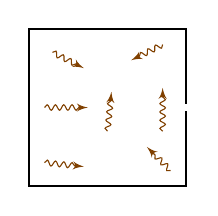
\begin{tikzpicture}[photon/.style={morange!50!black, decorate, decoration={snake, amplitude=1, segment length=3, post=lineto, post length=3}, -latex'}]
    \draw [thick] (0, 0) rectangle (2, 2);

    \draw [photon] (0.3, 1.7) -- +(0.4, -0.2);
    \draw [photon] (1, 0.7) -- +(0.05, 0.5);

    \draw [photon] (0.2, 0.3) -- +(0.5, -0.05);
    \draw [photon] (1.7, 0.7) -- +(0, 0.55);
    \draw [photon] (1.8, 0.2) -- +(-0.3, 0.3);
    \draw [photon] (0.2, 1) -- +(0.55, 0);
    \draw [photon] (1.7, 1.8) -- +(-0.4, -0.2);

    \fill [white] (1.95, 0.95) rectangle (2.05, 1.05);
  \end{tikzpicture}
\end{center}
Let's say this hole has area $A$, which is sufficiently small that it doesn't mess with what is going on in the box. How much energy do we expect the box to leak out of the hole?

For the purposes of this analysis, for a wave vector $\mathbf{k}$, we let $S(\mathbf{k})$ be the set of all photons with wave-vector within $\d^3 \mathbf{k}$ of $\mathbf{k}$. We further suppose $\mathbf{k}$ makes an angle $\theta$ with the normal to the hole.
\begin{center}
  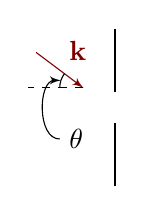
\begin{tikzpicture}
    \draw [thick] (0, 0) -- (0, 2);

    \fill [white] (-0.05, 0.8) rectangle (0.05, 1.2);

    \draw [mred, -latex'] (-1, 1.7) -- +(0.6, -0.45) node [pos=0.5, anchor=south west] {$\mathbf{k}$};

    \draw [dashed] (-0.4, 1.25) -- +(-0.7, 0);

    \draw (-0.7, 1.25) arc(180:143:0.3);:

    \draw (-0.7, 0.6) node [right] {$\theta$} edge [out=180, in=180, -latex'] (-0.685, 1.345);
  \end{tikzpicture}
\end{center}
What we want to know is what portion of $S(\mathbf{k})$ manages to get out of the hole, say in a time period $\d t$. To do so, we look at the following volume:
\begin{center}
  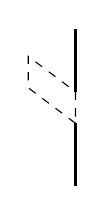
\begin{tikzpicture}
    \draw [thick] (0, 0) -- (0, 2);

    \fill [white] (-0.05, 0.8) rectangle (0.05, 1.2);

    \draw [dashed] (0, 0.8) -- (-0.6, 1.25) -- (-0.6, 1.65) -- (0, 1.2) -- cycle;
  \end{tikzpicture}
\end{center}
The volume of this box is $A c \cos \theta \;\d t$. So the proportion of energy that gets out is simply
\[
  \frac{A c \cos \theta}{V} \;\d t.
\]
We now write
\[
  E(|\mathbf{k}|) \;\d^3 \mathbf{k} = \text{total energy in $S(\mathbf{k})$}.
\]
Then the total energy leaving the hole in time $\d t$ as
\[
  \int_{\theta \in [0, \pi/2]} \d^3 \mathbf{k}\; \frac{A c \cos \theta}{V}\;\d t\; E(|\mathbf{k}|).
\]
To evaluate this integrate, we simply have to introduce polar coordinates, and we get
\[
  \frac{cA \;\d t}{V} \int_0^{2\pi} \int_0^{\pi/2} \d \theta \sin \theta \cos \theta \int_0^\infty \d |\mathbf{k}|\; |\mathbf{k}|^2 E(|\mathbf{k}|).
\]
The first two integrals give $2\pi$ and $\frac{1}{2}$ respectively, and we can rewrite the last integral back into Cartesian coordinates, and it is
\[
  \frac{1}{4\pi}\int \d^3 \mathbf{k}\; E(|\mathbf{k}|) = \frac{E}{4\pi}.
\]
Putting these all together, we find that the rate of energy emission is
\[
  \frac{1}{4} cA \mathcal{E} \;\d t.
\]
If we define the \term{energy flux} as energy per unit time per unit area leaving the hole, then the energy flux is given by
\[
  \frac{c}{4} \mathcal{E} = \sigma T^4,
\]
where
\[
  \sigma = \frac{\pi^2 k^4}{60 \hbar^3 c^2} \approx \SI{5.67e-8}{\joule\per\second\per\meter\squared\per\kelvin\tothe{-4}}.
\]
What was the point of computing this? We don't really care that much about the experimentalists. Suppose we had any black body, and we want to figure out how much radiation it is emitting. We imagine we put it inside that box. Then to the box, the surface of the black body is just like the hole we drilled through the box. So we know that the black body is absorbing $\sigma T^4$ energy per unit time per unit area.

But the system is in equilibrium, so the black body must emit the exact same amount of radiation out. So what we have derived is in fact how black bodies behave!

The best example of a black body we know of is the cosmic background microwave radiation of the universe. This is a black body radiation to incredibly high accuracy, with a temperature of $T = \SI{2.7}{\kelvin}$. This is the temperature of space.

Let's quickly calculate some other thermodynamic quantities we might be interested in. We have
\begin{align*}
  F &= - kT \log Z\\
  &= -\frac{VkT}{\pi^2 c^3}\int_0^\infty \d \omega\; \omega^2 \log (1 - e^{-\beta \hbar \omega})\\
  \intertext{Integrating by parts, we obtain}
  &= -\frac{V \hbar}{3\pi^2 c^3}\int_0^\infty \d \omega\; \frac{\omega^3 e^{-\beta \hbar \omega}}{1 - e^{-\beta \hbar \omega}}\\
  &= - \frac{V \hbar}{3\pi^2 c^3} \frac{1}{\beta^4 \hbar^4} \int_0^\infty \frac{x^3 \;\d x}{e^x - 1} \\
  &= - \frac{V \pi^2 k^4}{45 \hbar^3 c^3}T^4.
\end{align*}
The free energy is useful, because we can differentiate it to get pressure:
\[
  p = - \left(\frac{\partial F}{\partial V}\right)_T = \frac{E}{3V} = \frac{1}{3}\mathcal{E} = \frac{4\sigma}{3c} T^4.
\]
This is \term{radiation pressure}. Since $c$ is a big number, we see that radiation pressure is small.

We can also get the entropy from this. We compute
\[
  S = -\left(\frac{\partial F}{\partial T}\right)_V = \frac{16 V \sigma}{3c}T^3.
\]
Another quantity we can be interested in is the heat capacity, which is
\[
  C_V = \left(\frac{\partial E}{\partial T}\right)_V = \frac{16 V \sigma}{c} T^3.
\]
The classical/high temperature limit of black body radiation happens when $\hbar \omega \ll kT$. In this case, we have
\[
  \frac{1}{e^{\beta \hbar \omega} - 1} \approx \frac{1}{\beta \hbar \omega}.
\]
So we have
\[
  E(\omega) \;\d \omega \approx \frac{V \omega^2}{\pi^2 c^3}kT \;\d \omega \equiv E_{\mathrm{classical}} (\omega) \;\d \omega.
\]
This is known as the \emph{Rayleigh-Jeans law}. Note that there is no $\hbar$ in it. So it is indeed a classical result. It also agrees with equipartition of energy, as it does give $kT$ per normal mode of the electromagnetic field, with each mode viewed as a harmonic oscillator. We get $kT$ because here we have a potential. % think more about this.

However, this has the obvious problem that $E(\omega)$ is unbounded as $\omega \to \infty$. So if we tried to compute the total energy, then we get infinity. This is called the \term{ultraviolet catastrophy}. This showed that classical reasoning doesn't actually work at high energies, and this is what eventually led Planck to come up with Planck's constant.

\subsection{Phonons and the Debye model}
The next thing to discuss is something very similar to black body radiation, but has very different applications. We want to understand the heat capacity of solids. It turns out we can do using technology we have developed for the previous sections.

In the first example sheet, we studied a model of a solid, but treating it as some harmonic oscillators. We saw it was good at high temperatures, but rubbish at low temperatures. Here we are going to use a better model.

If we have a crystal lattice, then they vibrate, and these give sound waves in the crystal. In quantum mechanics, we know that light is made out of particles, called photons. Similarly, in quantum mechanics, sound is made up of ``particles'' called \term{phonons}. Similar to the case of photons, the energy of a phonon of frequency $\omega$ is
\[
  E = \hbar \omega,
\]
and the frequency of a phonon is described by a \term{dispersion relation} involving the wavevector $\mathbf{k}$.
\[
  \omega = \omega(\mathbf{k}).
\]
In general, this function is very complicated. We learn how to compute these in the IID Applications of Quantum Mechanics course, but we will not do that. 

Suppose the spacing in the crystal is $a$. Then if $|\mathbf{k}| a \ll 1$, then the dispersion relation becomes linear, and we have
\[
  \omega \approx |\mathbf{k}| c_s,
\]
where $c_s$ is the speed of sound in the solid. This is all very similar to photons, except we replace $c$ with $c_s$.

However, there is some important difference compared to photons. While photons have two polarizations, phonons have 3. Two of these are transverse, while the third is longitudinal. As one may know from the IID Waves course, they travel at different spaces, which we write as $c_T$ and $c_L$ for transverse and longitudinal respectively.

We now want to count the number of phonons, and obtain the density of states. Repeating what we did before, we find
\[
  g(\omega) \;\d \omega = \frac{V \omega^2}{2\pi} \left(\frac{2}{c_T^3} + \frac{1}{c_L^3}\right)\;\d \omega.
\]
This is valid for $|\mathbf{k}| a \ll 1$. Alternatively, we need $\omega a/ c_s  \ll 1$.

It is convenient to write this as
\[
  g(\omega) \;\d \omega = \frac{3 V \omega^2}{2\pi^2 \bar{c}_s^3}\;\d \omega,\tag{$*$}
\]
where
\[
  \frac{3}{\bar{c}_s^3} = \frac{2}{c_T^3} + \frac{1}{c_L^3}
\]
defines $\bar{c}_s$ as the \emph{average speed}.

The Debye model ignores the $|\mathbf{k}|a \ll 1$ assumption, and supposes it is also valid for $\omega a/c_3 \sim 1$.

There is another difference between photons and phonons --- for phonons, $\omega$ cannot be arbitrarily large. We know high $\omega$ corresponds to small wavelength, but if the wavelength gets too short, it is less than the separation of the atoms, which doesn't make sense. So we have a minimum possible wavelength set by the atomic spacing. Consequently, there is a maximum frequency $\omega_D$ ($D$ for $\emph{Debye}$).

We would expect the minimum wavelength to be $\sim a \sim \left(\frac{V}{N}\right)^{1/3}$. So we expect
\[
  \omega_D \sim \bar{c}_s \left(\frac{N}{V}\right)^{1/3}.
\]
Here we are assuming that the different speeds of sound are of similar orders of magnitude. So the total number of $1$-phonon states is
\[
  \int_0^{\omega_0} g(\omega) \;\d \omega = \frac{V \omega_0^2}{2\pi^2 \bar{c}_s^3}.
\]
This is the number of different ways the lattice can vibrate. In other words, the number of normal modes of the lattice.

\begin{claim}
  There are in fact $3N$ normal modes.
\end{claim}

\begin{proof}
  We consider the big vector
  \[
    \mathbf{X} = 
    \begin{pmatrix}
      \mathbf{x}_1\\
      \mathbf{x}_2\\
      \vdots\\
      \mathbf{x}_N
    \end{pmatrix},
  \]
  where each $\mathbf{x}_i$ is the position of the $i$th atom. Then the Lagrangian is
  \[
    L = \frac{1}{2} \dot{\mathbf{X}}^2 - V(\mathbf{X}),
  \]
  where $V$ is the interaction potential that keeps the solid a solid.

  We suppose $V$ is minimized at some particular $\mathbf{X} = \mathbf{X}_0$. We let
  \[
    \delta \mathbf{X} = \mathbf{X} - \mathbf{X}_0.
  \]
  Then we can write
  \[
    L = \frac{1}{2} m \delta \dot{\mathbf{X}}^2 - V_0 - \frac{1}{2} \delta \mathbf{X}^T \mathbf{V} \delta \mathbf{X} + \cdots,
  \]
  where $\mathbf{V}$ is the Hessian of $V$ at $\mathbf{X}_0$, which is a symmetric positive definite matrix since we are at a minimum. The equation of motion is then, to first order,
  \[
    m \delta \ddot{\mathbf{X}}  = - \mathbf{V} \delta \mathbf{X}.
  \]
  We assume that $\mathbf{X} = \Re(e^{i \omega t} \mathbf{Q})$ for some $\mathbf{Q}$ and $\omega$, and then this reduces to
  \[
    \mathbf{V} \mathbf{Q} = m \omega^2 \mathbf{Q}.
  \]
  This is an eigenvalue equation for $\mathbf{V}$. Since $\mathbf{V}$ is a $3n \times 3n$ symmetric matrix, it has $3N$ independent eigenvectors, and so we are done, and these are the $3N$ normal modes.

  If we wanted to, we can diagonalize $\mathbf{V}$, and then the system becomes $3N$ independent harmonic oscillators.
\end{proof}

If we accept that there are $3N$ normal modes, then this tells us
\[
  \frac{V \omega_0^2}{ 2\pi^2 \bar{c}_3^3} = 3N.
\]
Using this, we can determine
\[
  \omega_0 = \left(\frac{6 \pi^2 N}{V}\right)^{1/3} \bar{c}_s,
\]
which is of the form we predicted above by handwaving. We define
\[
  T_0 = \frac{\hbar \omega_0}{k},
\]
the \term{Debye temperature}. If we live in a frequency higher than this, then we are exciting the highest frequency phonons.

How high is this temperature? This depends only on $N, V$ and $\bar{c}_s$, and these are not hard to find. For example $T_0$ for lead is $\sim \SI{100}{\kelvin}$, since lead is a soft substance and speed is slow. On the other hand, $T_0 \sim \SI{2000}{\kelvin}$ for diamond, since it is hard.

We can compute partition functions for these, entirely analogous to that of photons. The only important difference is that we have that cutoff $\omega \leq \omega_0$. What we get is
\[
  \log Z = - \int_)^{\omega_0} \d \omega \; g(\omega) \log\left(1 - e^{-\beta \hbar \omega}\right).
\]
From the partition function, we can get the energy
\[
  E = -\left(\frac{\partial \log Z}{\partial  \beta}\right)_V  = \int_0^{\omega_0} \frac{\d \omega\; \hbar \omega g(\omega)}{e^{\beta \hbar \omega} - 1} = \frac{3V \hbar}{2\pi^2 \bar{c}_s^3} \int_0^{\omega_0} \frac{\d \omega\; \omega^3}{e^{\beta \hbar \omega} - 1}.
\]
Again we set $x = \beta \hbar \omega$. Then the limit becomes $x = T_0/T$. So the integral becomes
\[
  E = \frac{3V (kT)^4}{2\pi^3 (\hbar \bar{c}_s)^3} \int_0^{T_0/T} \frac{\d x\; x^3}{e^x - 1}.
\]
This is the same as the case of a photon, but the integral has a limit related to the temperature. This is integral not something we can investigate easily, but we can easily analyze what happens at extreme temperatures.
\begin{itemize}
  \item If $T \gg T_0$, then $x$ takes a very small range, and we can Taylor expand
    \[
      \int_0^{T_0/T}\frac{\d x\; x^3}{e^x - 1}= \int_0^{T_0/T} \d x\; (x^2 + \cdots) = \frac{1}{3} \left(\frac{T_0}{T}\right)^3.
    \]
    So we find that $E \propto T$, and
    \[
      C_V = \left(\frac{\partial E}{\partial T}\right)_V = \frac{V k^4 T_0^3}{2\pi^2(\hbar \bar{c}_s)^3} = 3 Nk.
    \]
    This agrees reasonably well with experiment, and is called the \term{Dulong-Petit law}. % check spelling
    This is also predicted by the Einstein's model. This is essentially just a consequence of the equipartition of energy, as there are $3N$ degrees of freedom, and we have $kT$ for each.
  \item If $T \ll T_0$, then we might as well replace the upper limit of the integral by infinity, and we have
    \[
      \int_0^{T_0/T} \frac{x^3}{e^x - 1} \approx \int_0^\infty \frac{x^3}{e^x - 1} = \frac{\pi^4}{15}.
    \]
    So we have $E \propto T^4$, which is exactly like photons. If we work out the heat capacity, then we find
    \[
      C_V = \frac{2\pi^2 V k^4}{5(\hbar \bar{c}_s)^3} T^3 = Nk \frac{12 \pi^4}{5}\left(\frac{T}{T_0}\right)^3.
    \]
    Remarkably, this $T^3$ behaviour also agrees with experiment for many substances, unlike the Einstein model.
\end{itemize}
% insert heat capacity C_V/Nk vs T, max at 3 approached near $T_D$.
This is pattern is observed for most solids. There is one important exception, which is for metals. In metals, we have electrons which are free to move in the lattice. In this case, they can also be considered to form a gas, and they are important at low temperatures.

Note that in the model, we made the assumption $\omega \approx |\mathbf{k}| c_s$. This is valid for $\omega \ll \omega_D$. Because of this, we would expect the Debye model to work at low temperatures $T \ll T_0$. At high temperature, we saw it also happens to works, but as we said, this is just equipartition of energy with $3N$ oscillators, and any model that involves $3N$ harmonic oscillators should give the same prediction.

\subsection{Quantum ideal gas}
Finally, we go back to talk about actual gases. Previously, for an ideal gas, we wrote
\[
  Z = Z_1^N,
\]
and we found there was a problem with entropy, and then we argued that we should have a factor of $\frac{1}{N!}$ there, because we over-counted identical states. However, it turns out this is still not quite true. This is really just an approximation that is valid at certain circumstances.

We let single particle states be $\bket{i}$, with energies $E_i$. For simplicity, we assume they are bosons. Let's consider the simplest non-trivial example, which is when $N = 2$. Then since we have two bosons, we know the states of the particles must be symmetric. So the possible states are of the form
\[
  \bket{i}\bket{i},\quad \frac{1}{\sqrt{2}} (\bket{i} \bket{j} + \bket{j} + \bket{i}),
\]
with $i \not= j$. Let's now calculate the partition function by summing over all these states. We have
\[
  Z = \sum_i e^{-\beta 2 E_i} + \frac{1}{2}\sum_{i \not= j}e^{-\beta (E_i + E_j)},
\]
where we had to divide by $2$ to avoid double counting. We compare this with
\[
  \frac{1}{2!} Z_1^2 = \frac{1}{2} \left( \sum_i e^{-\beta E_i} \right)\left(\sum_j e^{-\beta E_j}\right) = \frac{1}{2} \sum_i e^{-\beta 2E_i} + \frac{1}{2} \sum_{i \not= j} e^{-\beta(E_i + E_j)}.
\]
We see that the second parts are the same, but the first terms differ by a factor of $\frac{1}{2}$.

Fortunately, we have
\[
  Z \approx \frac{Z_1^2}{2!}
\]
if the probability of two particles being in the same one-particle state is negligible. Similarly, for $N$ particles, the approximation
\[
  Z = \frac{Z_1^N}{N!}\tag{$*$}
\]
is valid if the probability of $2$ or more particles being in the same state is negligible. This would be true if $\bra n_i\ket \ll 1$ for all $i$, where $n_i$ is the number of particles in $\bket{i}$. Under these circumstances, we can indeed use $(*)$. This is also true for Fermions, but we will not do those computations.

Last time, we fond
\[
  \bra n_i\ket = - \frac{1}{\beta} \frac{\partial \log Z}{\partial E_i} \approx -\frac{N}{\beta} \frac{\partial \log Z_1}{\partial E_i} = \frac{N}{Z_1} e^{-\beta E_i}
\]
for all $i$, where we used the approximation $(*)$ in deriving it.

For a monoatomic gas, we had
\[
  Z_i = \sum_I e^{-\beta E_i} \approx \int_0^\infty \d E \; g(e) e^{-\beta E} = \frac{V}{\lambda^3},
\]
where
\[
  \lambda = \sqrt{\frac{2\pi \hbar^2}{mkT}}.
\]
Note that this is exactly the same as the classical result, despite us using the integral approximation. Substituting this into our expression for $\bra n_i\ket$, we need
\[
  1 \gg \frac{N \lambda^3}{V} e^{-\beta E_i}
\]
for all $i$. So we need $\lambda \ll \left(\frac{V}{E}\right)^{1/3}$. So we see that this is valid when our gas is not too dense. And by our definition of $\lambda$, this is valid at high temperatures.

Recall that when we did diatomic gases classically, we had
\begin{align*}
  H &= H_{\mathrm{trans}} + H_{\mathrm{rot}} + H_{\mathrm{vib}}\\
  Z_1 &= Z_{\mathrm{trans}} + H_{\mathrm{rot}} + H_{\mathrm{vib}}
\end{align*}
We re-examine this in the quantum case.

We still have
\[
  H_{\mathrm{trans}} = \frac{\mathbf{p}^2}{2m}.
\]
So we find that
\[
  Z_{\mathrm{trans}} = \int_0^\infty \d E\; g(E) e^{-\beta E} = \frac{V}{\lambda^3},
\]
as before. So this part is unchanged.

We now look at the rotational part. We have
\[
  H_{\mathrm{rot}} = \frac{\mathbf{J}^2}{2I}.
\]
We know what the eigenvalues of $\mathbf{J}^2$ are. The energy levels are
\[
  \frac{\hbar^2 j(j + 1)}{2I},
\]
where $j = 0, 1, 2, \cdots$, and the degeneracy of each level is $2j + 1$. Using this, we can write down the partition function
\[
  Z_{\mathrm{rot}} = \sum_{j = 0}^\infty (2j + 1) e^{-\beta \hbar^3 j(j + 1)/2I}.
\]
Let's look at the high and low energy limits. If
\[
  kT \gg \frac{\hbar^2}{2I},
\]
then the exponents up there are small. So we can approximate the sum by an integral, 
\[
  Z_{\mathrm{rot}} \approx \int_0^\infty \d x\; (2x + 1) e^{-\beta \hbar^3 x(x + 1)/2I}.
\]
This fortunately is an integral we can evaluate, because
\[
  \frac{\d}{\d x} x(x + 1) = 2x + 1.
\]
So we find that
\[
  Z_{\mathrm{rot}} = \frac{2I}{\beta \hbar^2}.
\]
This is exactly what we saw classically. 

But if $kT \ll \frac{\hbar^2}{2I}$, all terms are exponentially suppressed except for $j = 0$. So we find
\[
  Z_{\mathrm{rot}} \approx 1.
\]
This is what we meant when we said the rotational modes are frozen out for low energy modes.

We can do the same thing for the vibrational modes of the degree of freedom. Recall we described them by harmonic oscillators. Recall that the energy levels are given by
\[
  E_n = k \omega\left(n + \frac{1}{2}\right).
\]
So we can write down the partition function
\[
  Z_{\mathrm{vib}} = \sum_{n = 0}^\infty e^{-\beta k\omega\left(n + \frac{1}{2}\right)} = e^{-\beta \hbar \omega/2} \frac{1}{1 - e^{-\beta \hbar \omega}} = \frac{1}{2 \sinh (\hbar \beta \omega/2)}.
\]
We can do the same thing as we did for rotational motion. Now the relevant energy scale is $\hbar \omega/2$.

At high temperatures $kT \gg \hbar \omega/2$, we can replace $\sinh$ by the first term in its Taylor expansion, and we have
\[
  Z_{\mathrm{vib}} \approx \frac{1}{\beta \hbar \omega}.
\]
On the other hand, at low temperatures, we have a sum of exponentially small terms, and so
\[
  Z_{\mathrm{vib}} \approx e^{-\beta \hbar \omega /2}.
\]
So we find that
\[
  E_{\mathrm{vib}} = - \frac{\partial}{\partial \beta}\log Z_{\mathrm{vib}} = \frac{\hbar \omega}{2}.
\]
So for $N$ molecules, we have
\[
  E_{\mathrm{vib}} \approx \frac{N \hbar \omega}{2}.
\]
But this is not measurable, as it is independent of $T$. So this doesn't affect the heat capacity. So the vibrational modes freeze out.

We can now understand the phenomenon we saw previously:
\begin{center}
  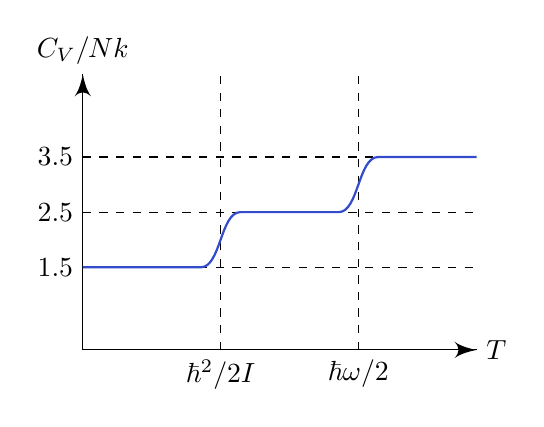
\begin{tikzpicture}[yscale=0.7]
    \draw [->] (0, 0) -- (5, 0) node [right] {$T$};
    \draw [->] (0, 0) -- (0, 5) node [above] {$C_V/Nk$};

    \draw [dashed] (1.75, 0) node [below] {$\hbar^2/2I$} -- +(0, 5);
    \draw [dashed] (3.5, 0) node [below] {$\hbar \omega/2$} -- +(0, 5);

    \draw [dashed] (0, 1.5) node [left] {$1.5$} -- +(5, 0);
    \draw [dashed] (0, 2.5) node [left] {$2.5$} -- +(5, 0);
    \draw [dashed] (0, 3.5) node [left] {$3.5$} -- +(5, 0);

    \draw [thick, mblue] (0, 1.5) -- (1.5, 1.5) .. controls (1.75, 1.5) and (1.75, 2.5) .. (2, 2.5) -- (3.25, 2.5) .. controls (3.5, 2.5) and (3.5, 3.5) .. (3.75, 3.5) -- (5, 3.5);;
  \end{tikzpicture}
\end{center}
Note that in theory it is certainly possible that the vibrational mode comes first, instead of what we drew. However, in practice, this rarely happens.

\subsection{Bosons}
In the previous derivation, we needed to assume that
\[
  \lambda = \sqrt{\frac{2\pi \hbar^2}{mkT}} \ll \left(\frac{V}{N}\right)^{1/2}.
\]
At \emph{very} low temperatures, this is no longer true. Then quantum effects become important. If there are no interactions between particles, then only one effect is important --- quantum statistics.
\begin{itemize}
  \item Bosons have integer spin, and the states have to be are symmetric with respect to interchange of $2$ particles. For example, photons are bosons.
  \item Fermions have spin $\frac{1}{2}$, and the states have to be antisymmetric, eg. $e, p, n$.
\end{itemize}
Since spins add up, atoms made from an even (odd resp.) number of electrons, protons and neutrons is a boson (fermion resp.). In an atom, since the charge is neutral, we know we have the same number of electrons and protons. So we are really counting the number of neutrons.

For example, hydrogen has no neutrons, so it is a boson. On the other hand, deuterium has 1 neutron, and so it is a fermion.

\subsubsection*{Bose--Einstein condensates}
We suppose we have bosons, and the single particles states are $\bket{r}$ with energy $E_r$. We let $n_r$ be the number of particles in $\bket{r}$. We assume the particles are indistinguishable, so to specify the state of the $n$-particle system, we just need to specify how many particles are in each $1$-particle state by
\[
  \{n_1, n_2, n_3, \cdots\}.
\]
Once we specify these numbers, then the energy is just
\[
  \sum_r n_r E_r.
\]
So we can write down the partition function in the canonical ensemble by summing over all possible states:
\[
  Z = \sum_{\{n_r\}} e^{-\beta \sum_s n_s E_s}.
\]
This is exactly the same as we had for photons. But there is one very important difference. For photons, the photon numbers are not conserved. But here the atoms cannot be destroyed. So we assume that the particle number is conserved. Thus, we are only summing over $\{n_r\}$ such that
\[
  \sum n_r = N.
\]
This makes it rather difficult to evaluate the sum. The trick is to use the grand canonical ensemble instead of the canonical ensemble. We have
\[
  \mathcal{Z} = \sum_{\{n_r\}} e^{-\beta \sum_s n_s (E_s - \mu)},
\]
and now there is no restriction on the allowed values of $\{n_i\}$. So we can factorize this sum and write it as
\[
  \mathcal{Z} = \prod_s \mathcal{Z}_s,
\]
where
\[
  \mathcal{Z}_s = \sum_{n_s = 0}^\infty e^{-\beta (E_s - \mu) n_s} = \frac{1}{1 - e^{-\beta(E_s - \mu)}}.
\]
For this sum to actually converge, we need $\mu < E_s$, and this has to be true for any $s$. So if the ground state energy is $E_0$, which we can always choose to be $0$, then we need $\mu < 0$.

Taking the logarithm, we can write
\[
  \log \mathcal{Z} = - \sum_r \log(1 - e^{-\beta (E_r - \mu)}).
\]
We can now compute the expectation values $\bar n_r\ket$. This is
\[
  \bra n_r \ket = - \frac{1}{\beta} \frac{\partial}{\partial E_r} \log \mathcal{Z} = \frac{1}{e^{\beta(E_r - \mu)} - 1}.
\]
This is called the \term{Bose-Einstein distribution}. This is the expected number of variables in the $1$-particle state $r$.

We can also ask for the expected total number of particles,
\[
  \bra N\ket = \frac{1}{\beta} \frac{\partial}{\partial \mu}\log \mathcal{Z} = \sum_r \frac{1}{e^{\beta(E_r - \mu)} - 1} = \sum_r \bra n_r\ket.
\]
Similarly, we have
\[
  \bra E\ket = \sum_r E_r \bra n_r\ket,
\]
as expected. As before, we will stop writing the brackets to denote expectation values.

It is convenient to introduce the \term{fugacity}\index{$z$}
\[
  z = e^{\beta\mu}.
\]
Since $\mu < 0$, we know
\[
  0 < z < 1.
\]
So far, what we have been doing is completely general, for arbitrary bosons. We now specialize to monoatomic, non-relativistic particles. We then replace the sums with the density of states
\[
  g(E) = \frac{V}{4\pi^2} \left(\frac{2m}{\hbar^2}\right)^{3/2} E^{1/2}.
\]
So we find
\[
  \log \mathcal{Z} = - \int_0^\infty \d E\; g(E) \log (1 - z e^{-\beta E}).
\]
The total number of particles is similarly
\[
  N = \int_0^\infty \d E\; \frac{g(E)}{z^{-1} e^{\beta E} - 1} = N(T, V, \mu).
\]
Now we are using the grand canonical ensemble just because it is convenient, not because we like it. So we hope that we can invert this relation to write % monotonicity?
\[
  \mu = \mu(T, V, N).\tag{$*$}
\]
So we can write
\[
  E = \int_)^\infty \d E\; \frac{E g(E)}{z^{-1} e^{\beta E} - 1} = E(T, V, \mu) = E(T, V, N),
\]
using $(*)$. As before, we have the grand canonical potential
\[
  pV = -\Phi = \frac{1}{\beta} \log \mathcal{Z} = -\frac{1}{\beta} \int_0^\infty \d E\; g(E) \log(1 - ze^{-\beta E}).
\]
Now there is a nice trick we can do. We integrate by parts, and by integrating $g(E)$ and differentiating the $\log$, we can obtain
\[
  pV = \frac{2}{3} \int_0^\infty \frac{\d E\; Eg(E)}{z^{-1} e^{\beta E} - 1} = \frac{2}{3} E.
\]
So if we can express $E$ as a function of $T, V, N$, then we can use this to give us an equation of state!

So what we want to do now is to actually evaluate those integrals, and then invert the relation we found. Unfortunately, these are not integrals we can do explicitly, so we can only do them at high and low temperature limits.

When we have high temperatures, we have $z \ll 1$ (it is not \emph{a priori} clear that this corresponds to high temperature. We will see that later). Then we find
\begin{align*}
  \frac{N}{V} &= \frac{1}{4\pi^2} \left(\frac{2m}{\hbar^2}\right)^{3/2} \int_0^\infty \frac{\d E\; E^{1/2}}{z^{-1} e^{\beta E} - 1}\\
  &= \frac{1}{4\pi^2} \left(\frac{2m}{\hbar^2}\right)^{3/2} \int_0^\infty \frac{\d E\; ze^{-\beta E} E^{1/2}}{1 - z e^{-\beta E}}\\
  &= \int_0^\infty \d E\; \frac{z e^{-\beta E}E^{1/2}}{1 - z e^{-\beta E}}\\
  &= \frac{1}{4\pi^2} \left(\frac{2m}{\hbar^2}\right)^{3/2} \frac{z}{\beta^{3/2}} \int_0^\infty \d x\; \sqrt{x} e^{-x}(1 + ze^{-x} + O(z^2))\\
  &= \frac{z}{\lambda^3} \left(1 + \frac{z}{2\sqrt{2}} + O(z^2)\right).
\end{align*}
To leading order, we must have
\[
  z = \lambda^3 \frac{N}{V},
\]
where $\lambda$ is again the de Broglie wavelength. So the statement that $z \ll 1$ is equivalent to
\[
  \lambda \ll \left(\frac{N}{V}\right)^{1/3},
\]
which is just our good old classical high-temperature limit.

Note that we know that $z = e^{\beta\mu}$. So we might that that if $T \to \infty$, then we have $\beta \to 0$, and we might have expected $z = e^{\beta \mu} \to 1$. But this is not what's happening. The reason is that we are keeping $N$ fixed here. So we have to let $\mu$ vary, and we see from this expression that
\[
  z \sim \lambda^3 \sim T^{-3/2}.
\]
At large $T$, we actually have $z \to 0$. So we know that $\mu \to -\infty$. So we have to be careful about what we are holding fixed when we take the limit.

We can do the same for the energy integral, and find
\begin{align*}
  \frac{E}{V} &= \frac{1}{4\pi^2} \left(\frac{2m}{\hbar^2}\right)^{3/2} \int_0^\infty \frac{\d E\; E^{3/2}}{z^{-1} e^{\beta E} - 1} \\
  &= \frac{1}{4\pi^2} \left(\frac{2m}{\hbar^2}\right)^{3/2} \frac{2}{\beta^{5/2}} \int_0^\infty \d x\; x^{3/2} e^{-x}(1 + z e^{-x} + O(z^2)\\
  &= \frac{3z}{2\lambda^3 \beta}\left(1 + \frac{z}{4\sqrt{2}} + O(z^2)\right).
\end{align*}
But we previously found $z$ as a function of $N/V$. Doing it order by order, we find
\[
  z = \lambda^3\frac{N}{V} \left(1 - \frac{1}{2\sqrt{2}} \frac{\lambda^3 N}{V} + O\left(\left(\frac{\lambda^3 N}{V}\right)^2\right)\right).
\]
Plugging this into our expression for $E/V$, we find that
\[
  E = \frac{3}{2} \frac{N}{\beta}\left(1 - \frac{1}{2\sqrt{2}} \frac{\lambda^3N}{V} + ..\right) + \left(\frac{1}{4\sqrt{2}} \frac{\lambda^3 N}{V} + \cdots\right).
\]
So we find that
\[
  pV = \frac{2}{3}E = NkT \left(1 - \frac{1}{4\sqrt{2}} \frac{\lambda^3 N}{V} + O\left(\left(\frac{\lambda^3N}{V}\right)^2\right)\right).
\]
We see that at leading order, we recover the \term{ideal gas law}. The first correction term is the \term{second Virial coefficient}\index{Virial coefficient!second}. These corrections are not coming from interactions, but quantum statistics.

\printindex
\end{document}
